\documentclass[a4paper,12pt]{article}
\usepackage{float}
\usepackage[polish]{babel}
\usepackage[cp1250]{inputenc}
\usepackage[T1]{fontenc}
\usepackage[dvips]{graphicx}
\usepackage{indentfirst}
\usepackage[urlcolor=blue, colorlinks=true, bookmarks=true, bookmarksnumbered=true]{hyperref}
\usepackage{fancyvrb}
\usepackage{times}
\usepackage{epsfig}
\usepackage{color}

\usepackage{fancyhdr} 
\pagestyle{fancy} 



\rfoot{SALOMON}
    


\title{Salomon}

\author{Nikodem Jura \emph{(\href{mailto:nico@icslab.agh.edu.pl}{nico@icslab.agh.edu.pl})}
        \\
        Krzysztof Rajda \emph{(\href{mailto:krzysztof@rajda.name}{krzysztof@rajda.name})}        
        }               
        

\begin{document}

\maketitle
%wylaczenie numerowania na I stronie
\thispagestyle{empty}

\begin{center}
\textcolor{blue}{\href{http://salomon.iisg.agh.edu.pl}{http://salomon.iisg.agh.edu.pl}}
\end{center}

\begin{center}
Prowadz�cy: mgr in�. Aleksander Byrski, dr in�. Marek Kisiel-Dorohinicki, 
\end{center}

\newpage

%spis tresci
\tableofcontents
\newpage

%reszta
\section{Wprowadzenie}

Salomon to system do wydobywania wiedzy z danych zgodnie z metodologi� \emph{Knowlege Mining}.
Odkrywanie wiedzy to proces iteracyjny, podzielony na etapy. W ka�dym tym etapie wiedza jest poddawana
obr�bce. Etapy te mog� tworzy� cykle. Na ka�dym takim etapie proces odkrywania mo�e by� ukierunkowany zgodnie
z wymaganiami u�ytkownika. Ka�dy etap tworzy odr�bn� ca�o��. 

W Salomonie reprezentacj� etapu jest \emph{zadanie} (Task). Ka�de zadanie mo�e posiada� kilka nast�pnik�w i kilka
poprzednik�w. Ujmuj�c rzecz pro�ciej, zadania mog� by� zorganizowane w postaci grafu. 

Zadanie zdefiniowane jest jako tr�jka:
\begin{itemize}
	\item algorytm(dostarczany w postaci wtyczki, czyli \emph{pluginu}))
	\item dane steruj�ce algorytmem
	\item dane wej�ciowe, z kt�rych algorytm b�dzie wydobywa� wiedz�
\end{itemize}

Zadanie nie musi si� ogranicza� do danych, kt�re otrzyma�o z poprzedniego zadania. Ka�de zadanie ma
dost�p do ca�ej aktualnie zgromadzonej wiedzy i do wszystkich danych.

Na wej�ciu lub wyj�ciu ka�dego zadania mog� pojawi� si� dane (w przypadku algorytm�w, kt�re
dokonuj� selekcji/segregacji danych), wiedza lub obie te rzeczy naraz.

\begin{itemize}
	\item dane \begin{math}\Rightarrow \end{math} dane - najcz�ciej taki przypadek zdarza si� kiedy chcemy stworzy�
	zbiory treningowe lub zbiory testuj�ce
	\item dane \begin{math}\Rightarrow \end{math} wiedza - typowy przyk�ad wyszukiwania wiedzy: dostajemy dane, uzyskujemy wiedz�
	\item wiedza+dane \begin{math}\Rightarrow \end{math} dane - przypadek taki zachodzi kiedy chcemy wykorzysta� zgromadzon� wiedz� na dostarczonych danych
	\item wiedza \begin{math}\Rightarrow \end{math} wiedza
\end{itemize}

Celem tego projektu jest stworzenie przyjaznego �rodowiska do tworzenia, kontrolowania i efektywnego wykonywania zada� oraz przechowywania zgromadzonej wiedzy.

Salomon sk�ada si� z dw�ch zasadniczych cz�ci - pierwsz� z nich
stanowi platforma. Tworz� j�:
\begin{itemize}
	\item silnik, kt�rego zadaniem jest zarz�dzanie i~uruchamianie
zada�
	\item magazyn s�u��cy do przechowywania wiedzy
\end{itemize}

Druga cz�� to zbi�r wtyczek, dostarczaj�cych logik� potrzebn� do skonfigurowania, wykonania i~wy�wietlenia rezultat�w
zadania. System jest otwarty - oznacza to, �e jego funkcjonalno�� mo�e by� w �atwy spos�b rozszerzana poprzez dostarczenie nowych wtyczek.

\begin{figure}[htb]
	\centering
		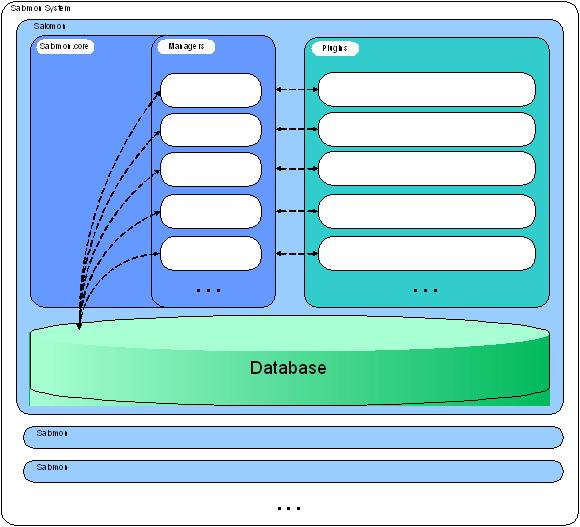
\includegraphics[width=0.90\textwidth]{img/uml/arch.jpg}
	\caption{Architektura systemu}
\end{figure}


\pagebreak
Podstawowe za�o�enia projektowe:
\begin{itemize}
    \item ca�a funkcjonalno�� w pluginach. J�dro systemu ma by� jak najmniejsze.
    Jego zadaniem jest stworzenie �rodowiska do realizacji logiki dostarczanej we wtyczkach
    \item otwarta~architektura. Wprowadzenie warstwy po�redniej pomi�dzy baz� danych~a wtyczkami.
    Jej zadaniem jest ukrycie sposobu organizacji danych przez
    wtyczkami. Otwarto��~architektury polega na mo�liwo�ci rozszerzenia tej warstwy
    \item niezale�no�� od platformy. System ma by� niezale�ny od platformy, mo�liwie �atwo przenaszalny.
    Poszczeg�lne cz�ci systemu mog� by� uruchamiane na r�nych
    platformach.
    \item mo�liwo�� wykorzystywania rezultat�w poprzednich zada� przez kolejne
    \item �atwa~adaptacja funkcjonalno�ci zawartej w \emph{Vinlenie}.
    Projekt powsta� jako platforma uruchomieniowa dla logiki zaimplementowanej w programie \emph{Vinlen},
    tworzonego pod kierownictwem prof. Ryszarda Michalskiego.    
\end{itemize}


Salomon ma na celu wyeliminowanie ogranicze� oryginalnego
\emph{Vinlena} poprzez wprowadzenie:

\begin{itemize}
    \item kolejkowania zada�
    \item rozproszenia
    \item r�wnoleg�o�ci
    \item rozszerzalno�ci (mechanizm wtyczek)
    \item przeno�no�ci (\emph{Java},\emph{Firebird})
\end{itemize}
\section{Koncepcja systemu}

Przedstawiona poni�ej koncepcja zak�ada stworzenie systemu o~nazwie \emph{Salomon}, kt�ry stanowi� b�dzie odpowiedz na opisane wcze�niej wymagania. 

Podstawowym za�o�eniem przy�wiecaj�cym opracowywaniu tego �rodowiska jest koncepcja zadaniowo�ci. \\
Odkrywanie wiedzy to~proces iteracyjny, podzielony na etapy. Etapy te mog� tworzy� cykle.
W ka�dym tym etapie wiedza jest poddawana obr�bce. 
Na ka�dym takim etapie proces odkrywania mo�e by� ukierunkowany zgodnie
z wymaganiami u�ytkownika. Ka�dy etap tworzy odr�bn� ca�o��. 
Cz�� etap�w jest roz��czna, zatem mog� by� wykonywane wsp�bie�nie. 
Architektura Salomona pozwala na rozproszone, a~co za tym idzie 
-- zr�wnoleglenie wykonywania takich roz��cznych etap�w oraz na synchronizacj� ich wynik�w.

Jednym z~istotnych atut�w systemu jest mo�liwo�� elastycznego definiowania
przebiegu pracy systemu w~kategoriach tzw.\ \emph{zada\'n}.
Ekstrakcja wiedzy to~proces, kt�ry mo�e
by� podzielony na etapy -- w~ka�dym etapie wiedza jest poddawana
pewnej obr�bce (np. dyskretyzowane s� atrybuty, tworzone s�
regu�y, wiedza jest testowana). Poniewa� ka�dy etap tworzy odr�bn�
ca�o��, a~cz�� etap�w jest od siebie niezale�na, zatem mog� by�
one wykonywane wsp�bie�nie.

\label{lab:tasks}
Zadanie to~podstawowa jednostka reprezentuj�ca obliczenia.
Zdefiniowane jest ono jako: 
$$
z=(a, p, we, wy)
$$
gdzie:
\begin{itemize}
    \item $a$ jest algorytmem, dostarczanym do systemu w~postaci komponentu --
    wtyczki,
    \item $p$ reprezentuje parametry algorytmu,
    \item $we$ i~$wy$ oznaczaj� odpowiednio informacje wej�ciowe i
    wyj�ciowe algorytmu.
\end{itemize}
Wej�cie i~wyj�cie mo�e mie� posta� danych (w~przypadku algorytm�w,
kt�re dokonuj� np. selekcji danych), wiedzy (np. wygenerowane
regu�y) lub danych i~wiedzy naraz (np.\ regu�y i~wyj�tki dla
nich).

Wyj�cie jednego zadania mo�e by� wej�ciem pewnej liczby nast�pnych
zada�. Aby zadanie mog�o zosta� wykonane, wszystkie zadania od
kt�rych zale�y musz� by� wykonane wcze�niej. Powi�zane zadania
mog� by� przedstawione w~postaci grafu skierowanego. Taki graf z
zaznaczonym zadaniem pocz�tkowym tworzy \emph{program}. Dodatkowo,
ka�da kraw�d� mo�e mie� przypisany warunek, kt�ry jest wymagany,
aby sterowanie zosta�o przekazane wzd�u� tej kraw�dzi. Tak
zdefiniowany program mo�e by� �atwo prezentowany u�ytkownikowi w~postaci
graficznej. 

\label{lab:agents}
W systemie mo�na definiowa� agent�w, kt�rzy reaguj� na zmiany w~danych i/lub
wiedzy. Obecnie jest jedynym rodzajem zdarzenia, kt�ry mo�e wywo�a� akcje
jest pojawienie si� nowych danych w~systemie. Jednak w~przysz�o�ci istnieje
mo�liwo�� dodania kolejnych rodzaj�w zdarze� takich jak np. wygenerowanie
wiedzy przez innego agenta. W~reakcji na wyst�pienie zdarzenia system
wykonuje zdefiniowany program, za pomoc� kt�rego mo�na przyk�adowo sprawdzi� poprawno�� aktualnej zgromadzonej wiedzy na nowych danych, czy wygenerowa� now�.
% (np.\ na dodanie nowego rekordu do danych treningowych, czy
%wygenerowanie wiedzy przez innego agenta).
%W~systemie b�dzie mo�na tak�e
%definiowa� agent�w, kt�rzy reagowa� b�d� na zmiany w~danych i/lub wiedzy
%(np.\ na dodanie nowego rekordu do danych treningowych, czy
%wygenerowanie wiedzy przez innego agenta).


%W~systemie b�dzie mo�na tak�e
%definiowa� agent�w, kt�rzy reagowa� b�d� na zmiany w~danych i/lub wiedzy
%(np.\ na dodanie nowego rekordu do danych treningowych, czy
%wygenerowanie wiedzy przez innego agenta).

Bardzo wa�nym mechanizmem Salomona jest mo�liwo�� tworzenia powi�za� 
mi�dzy poszczeg�lnymi zadaniami. 
Wynik jednego zadania mo�e pos�u�y� jako wej�cie nast�pnego. 
Salomon w~tym celu dostarcza �rodowisko. Wtyczka w~trakcie wykonywania zadania 
opr�cz dost�pu  do menad�er�w posiada r�wnie� dost�p do �rodowiska, 
z kt�rego mo�e pobra� warto�ci zmiennych �rodowiskowych. 
Dane �rodowisko tworzone jest na pocz�tku wykonania listy zada� 
i przekazywane jest kolejno do nast�pnego zadania. 
Wtyczka w~trakcie pracy mo�e modyfikowa� �rodowisko poprzez dodawanie, 
usuwanie oraz edycj� poszczeg�lnych zmiennych. W~ten spos�b poszczeg�lne 
zadania mog� mi�dzy sob� przekazywa� informacje. Zmienne �rodowiskowe, 
podobnie jak ustawienia i~rezultaty zada�, s� persystentne, a~co za tym 
idzie potrzebny jest mechanizm serializacji i~deserializacji.

Mechanizm tworzenia zmiennych �rodowiskowych opiera si� na tym samym modelu
co tworzenie ustawie� i~rezultat�w dla zada�. Mo�liwo�� tworzenia zmiennych
�rodowiskowych przez wtyczki mo�e rodzi� wiele problem�w z~zapewnieniem 
kompatybilno�ci mi�dzy r�nymi wersjami wtyczek, komunikuj�cych si� ze sob�, 
dlatego te� aby unikn�� takich problem�w, ka�da wtyczka zmuszona b�dzie 
dostarczy� opis zmiennych, kt�re mo�e tworzy�.

% TODO: przeniesc do implementacji -- dodac cos o~serializacji
%Mechanizm serializacji opiera si� na agregacji typ�w prostych 
%i innych typ�w z�o�onych. Za~pomoc� takich element�w, 
%programista mo�e stworzy� hierarchiczne struktury danych.
%Wprowadzenie takiego mechanizmu podyktowane jest potrzeb� ukrycia
%przed programist� sposobu zapisu danych w~bazie lub w~pliku. 
%Dostarczenie sp�jnego modelu serializacji danych pozwala na 
%niewidoczny dla wtyczek spos�b podmiany implementacji na bardziej 
%efektywn� itp. Mechanizm ten mo�e okaza� si� r�wnie� po�yteczny 
%po dodaniu do Salomona mo�liwo�ci definiowania zada� w~pliku (np. XML).
%Serializacja danych mo�e odbywa� si� do wielu format�w 
%np. XML, CSV, tabel w~bazie danych itp.

Na wej�ciu lub wyj�ciu ka�dego zadania mog� pojawi� si� dane (w przypadku algorytm�w, kt�re
dokonuj� selekcji/segregacji danych), wiedza lub obie te rzeczy naraz (rys. \ref{fig:WorkflowGraph} i~rys. \ref{fig:WorkflowSequental}).

\begin{itemize}
	\item \begin{math} dane \Rightarrow  dane \end{math} - najcz�ciej taki przypadek zdarza si� kiedy chcemy stworzy�
	zbiory treningowe lub zbiory testuj�ce
	\item \begin{math} dane \Rightarrow wiedza \end{math} - typowy przyk�ad wyszukiwania wiedzy: dostajemy dane, uzyskujemy wiedz�
	\item \begin{math} wiedza + dane \Rightarrow  dane \end{math} - przypadek taki zachodzi kiedy chcemy wykorzysta� zgromadzon� wiedz� na dostarczonych danych
	\item wiedza \begin{math}\Rightarrow \end{math} wiedza
\end{itemize}

\begin{figure}[H]
	\centering
		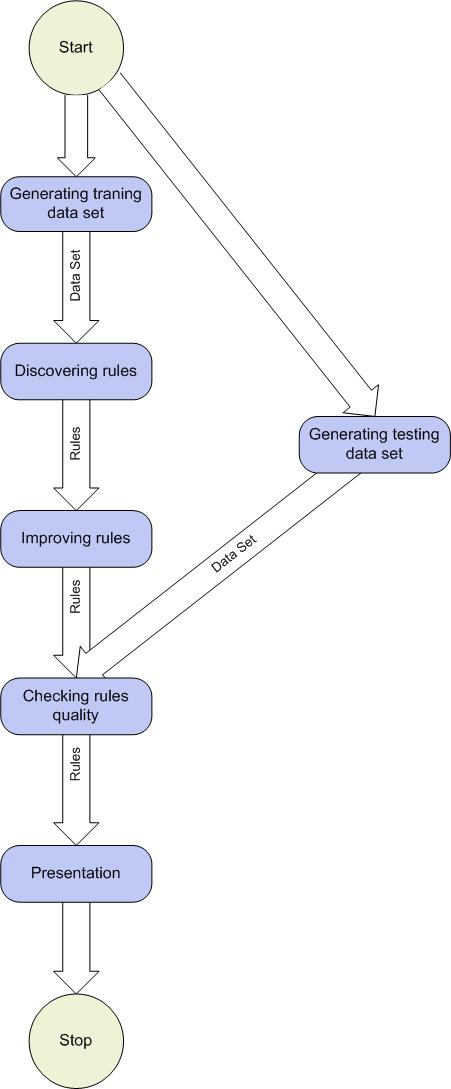
\includegraphics[height=0.90\textheight]{img/salomon/concept/WorkflowGraph.jpg}
	\caption{Przep�yw danych}		
	\label{fig:WorkflowGraph}
\end{figure}


\begin{figure}[H]
	\centering
		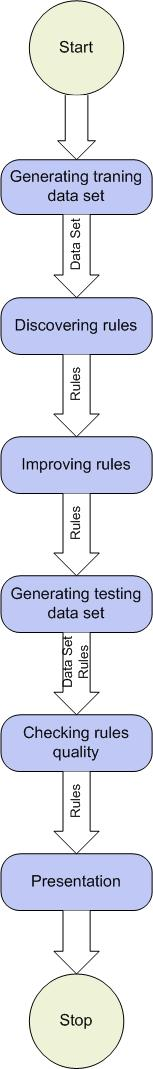
\includegraphics[height=0.90\textheight]{img/salomon/concept/WorkflowSequental.jpg}
	\caption{Sekwencyjny przep�yw danych}
	\label{fig:WorkflowSequental}
\end{figure}


\section{Funkcjonalno��}

Ca�a funkcjonalno�� \emph{Salomona} podporz�dkowana jest tworzeniu zada�. Operacje podstawowe, takie jak np. tworzenie projekt�w czy definiowanie wtyczek s�u�� jedynie stworzeniu �rodowiska, w~kt�rym mog� by� wykonywane zadania. Z~kolei operacje administracyjne pozwalaj� na~zaawansowane zarz�dzanie platform� i~mog� by� u�yteczne dla u�ytkownik�w bardzo dobrze znaj�cych wewn�trzn� struktur� systemu.

\subsection{Operacje podstawowe}

\subsubsection{Operacje na~obiekcie Solution}
\label{lab:solution}

Terminem \textbf{Solution} okre�lamy struktur� grupuj�c� projekty.
W obr�bie jednego obiektu \emph{Solution} zgrupowane s� projekty, 
kt�re operuj� na~tym samym zewn�trznym �r�dle danych.
W obecnej wersji s� to~zewn�trzne bazy danych. Obiekt ten przechowuje 
informacje niezb�dne do~uzyskania dost�pu do~danych,
a wi�c parametry po��czenia i~lokalizacj� bazy danych.

Mo�na na~nim wykona� nast�puj�ce operacje:

\begin{itemize}
	\item Utworzenie nowego
		
	Zadanie to~wymaga konfiguracji, w~szczeg�lno�ci wskazania lokacji bazy danych i~innych parametr�w po��czenia.
		
	\item Edycja istniej�cego
	
	System pozwala na~wyb�r aktualnego \emph{Solutiona}. Mo�na to~zrobi� przy uruchamianiu programu, kiedy to~trzeba albo wskaza� istniej�cy \emph{Solution} albo utworzy� nowy, b�d� w~dowolnym innym momencie, poprzez wyb�r odpowiedniej opcji z~menu. Tylko w~ten spos�b mo�na zmieni� parametry ju� istniej�cego obiektu \emph{Solution}.	

\end{itemize}

\subsubsection{Operacje na~projektach}
\label{lab:project}

\textbf{Projekty} s�u�� do~grupowania zada� w~obr�bie tego samego obiektu \emph{Solution}.			
W ramach projekt�w zapisywana jest konfiguracja systemu przed wykonaniem grupy zada�.
Zadania te grupowane s� w~formie grafu skierowanego acyklicznego.
Struktura taka opisuje zestaw zada�, kt�re musz� zosta� wykonane w~okre�lonej kolejno�ci
aby uzyska� zamierzony efekt. Przyk�adowo, aby stworzy� i~wy�wietli� drzewo decyzyjne,
mo�na zdefiniowa� zadania dla poszczeg�lnych krok�w, a~wi�c wybrania zbioru danych, zdefiniowania zbioru atrybut�w,
skonfigurowania algorytmu tworz�cego drzewo, czy wreszcie jego wizualizacji.
Projekty mog� by� u�yte wielokrotnie dla r�nych danych i~r�nej konfiguracji zada�. 

Operacje na~projekcie:		
	\begin{itemize}	
		\item Utworzenie projektu
		
		Nowy projekt tworzony jest automatycznie podczas uruchomienia systemu. Mo�na te� wymusi� utworzenie nowego projektu poprzez wyb�r odpowiedniej opcji z~menu.
		
		\item Edycja bie��cego projektu
		
		Operacja ta pozwala na~zmian� podstawowych informacji o~projekcie, a~wi�c jego nazwy i~dodatkowych informacji.
			
		\item Uruchomienie projektu
		
        Akcja ta powoduje wykonanie zada� zgromadzonych w~tym projekcie. Wykonanie tej akcji wymaga wcze�niejszej konfiguracji w~postaci specyfikacji listy zada� do~wykonania oraz ich indywidualnej konfiguracji.
        
		\item Konfiguracja agent�w

		Do projektu mo�na przypisa� agenty (\ref{lab:agents}), kt�rzy mog� reagowa� na~zmiany w~danych, na~kt�rych operuj� zadania w~obr�bie danego projektu. W~przypadku zmiany tych danych aganci mog� spowodowa� ponowne uruchomienie zada� na~zaktualizowanych danych.

	\end{itemize}
	
\subsubsection{Operacje na~wtyczkach}
\label{lab:plugin}
\emph{Wtyczka} to~zewn�trzny program odpowiedzialny za~wykonanie konkretnego zadania.
Mo�e zawiera� algorytm obliczeniowy, ale nie tylko -- wtyczki mog� te� s�u�y�
np. do~definiowania nowych zbior�w danych czy do~wy�wietlania drzew decyzyjnych
w formie graficznej. Ka�da wtyczka mo�e by� skonfigurowana przed wykonaniem jej 
g��wnego zadania. Za~obs�ug� konfiguracji odpowiada platforma, tw�rca wtyczki musi
jedynie dostarczy� komponent�w pozwalaj�cych na~skonfigurowanie ustawie� wtyczki
z poziomu graficznego interfejsu u�ytkownika.
Wtyczki nie s� integraln� cz�ci� systemu. W~razie konieczno�ci mog� by� pobierane 
z okre�lonej zdalnej lokalizacji.
Wtyczki zawieraj� algorytmy, kt�re mog� by� wykonywane przez platform� w~ramach poszczeg�lnych zada�.
S� one podstawowymi komponentami, kt�re rozszerzaj� mo�liwo�ci systemu.

	\begin{itemize}
	
		\item Dodanie
		
			Operacja ta pozwala na~zdefiniowanie nowej wtyczki poprzez wskazanie odpowiedniego pliku j� reprezentuj�cego.
		
		\item Edycja
		
			Za pomoc� tej operacji mo�na zmienia� nazw� i~opis wcze�niej zdefiniowanej wtyczki.
		
		\item Usuni�cie
		
			Pozwala na~usuni�cie wtyczki z~systemu.
					
	\end{itemize}


\subsection{Operacje na~zadaniach}
\label{lab:task}
Definiowanie zada� do~wykonania nale�y do~podstawowych funkcji systemu, dlatego w~obecnej wersji ich definiowanie i~konfigurowanie zosta�o znacznie rozbudowane.

\textbf{Zadanie} to~podstawowa jednostka obliczeniowa.
Zawiera algorytm, kt�ry ma zosta� wykonany oraz jego ustawienia.
Algorytm dostarczany jest w~formie wtyczki. Szerszy opis zada� znajduje si� w~rozdziale \ref{lab:tasks}.

Pierwsze wersje \emph{Salomona} pozwala�y jedynie na~definiowanie liniowej listy zada�.
Dlatego, aby umo�liwi� tworzenie bardziej zaawansowanych struktur zada� zosta� stworzony nowy komponent oparty o~bibliotek� \emph{Jung}.
Zadania reprezentowane w~nim s� jako w�z�y w~grafie skierowanym acyklicznym. Kraw�dzie reprezentuj� przep�yw sterowania (wiedzy/danych).

Aby dane zadanie mog�o by� wykonane wszystkie zadania od kt�rych zale�y musz� by� wykonane wcze�niej.
W obecnej wersji acykliczno�� grafu jest wymagana, aby zapewni�, �e wykonanie programu si� zako�czy.
W kolejnych wersjach planowane jest umo�liwienie dodawania warunk�w na~kraw�dzie, a~tym samym
mo�liwo�ci tworzenia cykli, kt�re zostan� przerwane, je�li zostanie spe�niony odpowiedni warunek.

Obecnie obs�ugiwane s� nast�puj�ce operacje na~zadaniach:

		\begin{itemize}
			\item Dodanie
			
			Dodanie zadania polega na~zdefiniowaniu jego nazwy i~wskazaniu wtyczki, kt�ra zawiera odpowiedni algorytm.
			
			\item Usuni�cie
			
            Akcja usuwa aktualnie zaznaczone zadnie.             
            
            \item Okre�lanie kolejno�ci wykonania
            
            Zadania wykonywane s� tak, jak zosta�y po��czone kraw�dziami. Strza�ki na~kraw�dziach okre�laj� kolejne zadania do~wykonania. W�z�y grafu, kt�re reprezentuj� poszczeg�lne zadania mog� by� w~dowolny spos�b przemieszczane oraz ��czone.
            
        \item Definiowanie ustawie� zadania
        
        Ka�de zadanie mo�e by� skonfigurowane przed wykonaniem. Spos�b konfiguracji zale�y od poszczeg�lnych wtyczek i~to one dostarczaj� komponenty pozwalaj�ce na~skonfigurowanie danej wtyczki.
        
        \item Uruchomienie zada�
        
        Po zdefiniowaniu kolejno�ci wykonania zada� mo�na je uruchomi� -- zadania zostan� przetworzone, a~ich wyniki zapisane w~bazie danych.
        
  		\item Przegl�danie rezultat�w
        
        Ka�de wtyczka, kt�rej algorytm przetwarzany jest w~ramach zadania, sama specyfikuje jak b�dzie prezentowa� swoje wyniki. Zdaniem platformy jest jedynie zapewnienie mo�liwo�ci wy�wietlenia zwr�conych przez wtyczk� danych.
		\end{itemize}

\subsection{Administracja}

\emph{Salomon} dostarcza narz�dzi u�atwiaj�ce administrowanie danymi zgromadzonymi w~systemie -- mo�liwe jest przegl�danie wszystkich zapisanych w~bazie danych obiekt�w, a~zaawansowani u�ytkownicy mog� wykona� dowolne operacje bezpo�rednio na~bazie danych za~pomoc� \emph{SQLConsole}.
	
	\begin{itemize}
            
		\item Przegl�danie obiekt�w w~systemie
		
		W celach administracyjnych mo�liwe jest przegl�danie obiekt�w w~taki spos�b, w~jaki zapisane s� w~bazie danych oraz na~ich usuni�cie.
			
		\item Zaawansowane operacje
		
		Do bardziej zaawansowanych operacji na~bazie danych przeznaczona jest specjalna konsola (\emph{SQLConsole}), kt�ra pozwala na~wykonanie dowolnych operacji na~bazie danych.
		
	\end{itemize}	


Przedstawiona w~poprzednim rozdziale koncepcja systemu pozwala na elastyczne rozszerzanie jego mo�liwo�ci dzi�ki zastosowaniu architektury komponentowej.
Poni�ej przedstawiono elementy adekwatnej implementacji. Jej  g��wn� cz�� stanowi platforma, kt�rej mo�liwo�ci mog� by� rozszerzane za pomoc� wtyczek.

\section{Platforma}
\label{lab:platform-interfaces}

Trzonem systemu jest platforma, kt�ra
dostarcza podstawowej funkcjonalno�ci umo�liwiaj�cej prac� ca�ego
systemu, �aduje odpowiedni kontroler, wczytuje wtyczki, uruchamia
zadania. Odpowiada tak�e za komunikacje mi�dzy innymi instancjami \emph{Salomona}.

\begin{figure}[H]
	\centering
		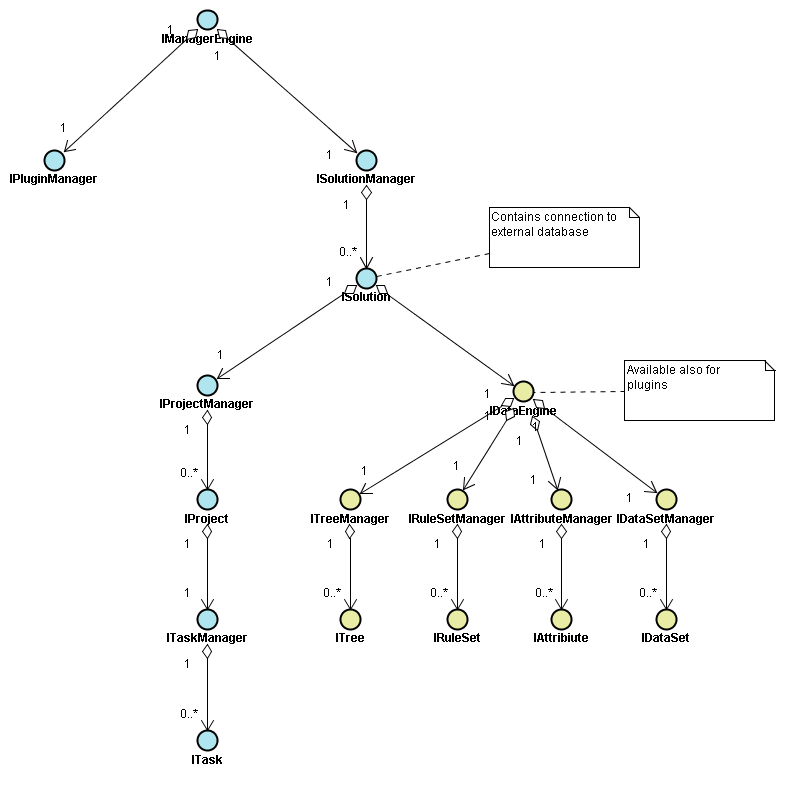
\includegraphics[width=1.00\textwidth]{img/salomon/uml/manager_engine.png}
	\caption{G��wne interfejsy platformy}
	\label{fig:core}
\end{figure}

Interfejsy maj�ce w~nazwie s�owo \emph{Manager} pe�ni� szczeg�ln� funkcj� 
-- najcz�ciej odpowiadaj� za zarz�dzanie innymi interfejsami, np. \emph{IPluginManger} zarz�dza wtyczkami, \emph{IProjectManger} -- projektami.
Dostarczaj� one zestawu metod pozwalaj�cych na wygodne zarz�dzanie obiektami,
ich tworzenie, modyfikowanie, czy usuwanie.
Wszystkie menad�ery maj� analogiczn� funkcjonalno�� -- ka�dy z
nich pozwala na stworzenie nowego obiektu, kt�rym zarz�dza (nie ma innej
mo�liwo�ci ich stworzenia, ni� przez metody udost�pniane przez menad�era), jego
zesk�adowanie w~bazie danych, zwr�cenie wszystkich zarz�dzanych obiekt�w, czy
te� pojedynczego, bazuj�c na unikalnym identyfikatorze oraz usuni�cie konkretnego obiektu.

Menad�ery nie s� dost�pne bezpo�rednio z~platformy, ale
przekazywane s� wtyczkom za pomoc� interfejsu \emph{IDataEngine}.
Wtyczka, zale�nie od potrzeb, pobiera za pomoc� tego interfejsu potrzebny jej menad�er i~za jego
po�rednictwem zarz�dza zbiorem danych, atrybut�w lub drzewem decyzyjnym.

\subsection{IManagerEngine}

Interfejs ten zapewnia dost�p do om�wionych poni�ej menad�er�w.

\paragraph{IPluginManager}

Interfejs \emph{IPluginManager} zarz�dza wtyczkami (por. \ref{lab:plugin}). Pozwala na zapisanie informacji o~nowej wtyczce
(jej nazwie, lokalizacji) oraz na pobranie listy dost�pnych wtyczek.
Mog� one by� �adowane ze zdalnej lokalizacji, a~wi�c zadaniem tego
menad�era jest tak�e zarz�dzanie pobieraniem i~buforowaniem wtyczek pobranych
z zewn�trznych �r�de�.

\paragraph{ISolutionManager}

\emph{ISolutionManager} zarz�dza obiektami implementuj�cymi interfejs \emph{ISolution} (por. \ref{lab:solution}).

\paragraph{IProjectManager}

Interfejs ten umo�liwia zarz�dzanie projektami zdefiniowanymi dla
okre�lonego obiektu \emph{ISolution} (por. \ref{lab:project}) .

\paragraph{ITaskManager}

Interfejs ten dostarcza funkcjonalno�ci umo�liwiaj�cej zarz�dzanie zadaniami (por. \ref{lab:tasks}) dla konkretnego projektu. Opr�cz standardowych operacji wsp�lnych dla wszystkich menad�er�w, jego zadaniem jest tak�e zapewnienie poprawnej konfiguracji, nadz�r nad wykonaniem oraz zachowanie informacji
o przebiegu przetwarzania zada�.

\subsection{IDataEngine}
\label{lab:data_engine}

Obiekt implementuj�cy ten interfejs przekazywany jest wtyczkom podczas ich wykonania.
Za pomoc� pobieranych z~niego menad�er�w jak na przyk�ad \emph{IDataSetManager} 
czy \emph{ITreeManager}
wtyczki mog� operowa� na danych znajduj�cych si� w~bazie.
Udost�pnienie wtyczkom jedynie interfejs�w do operowania na danych pozwala
na ukrycie sposobu sk�adowania danych przed tw�rcami wtyczek i~ich uniezale�nienie si�
od implementacji. W~obecnej wersji dane przechowywane s� w~relacyjnej bazie danych, ale nic nie stoi 
na przeszkodzie, by w~przysz�o�ci przechowywa� je w~inny spos�b, np. w~plikach tekstowych o~ustalonym formacie
czy bazie \emph{LDAP}. Tw�rcy wtyczek nie musz� troszczy� si� o~to, jak dane s� przechowywane, gdy� implementacja
interfejs�w dostarczona jest przez platform�.
Co wi�cej, raz napisane wtyczki b�d� dzia�a� tak�e z~nowszymi jej wersjami,
pod warunkiem zachowania dotychczasowych interfejs�w.

W obecnej wersji wtyczki mog� operowa� na zbiorach danych, atrybutach oraz 
drzewach decyzyjnych odpowiednio za pomoc� interfejs�w \emph{IDataSetManager}, \emph{IAttributeManager} i~\emph{ITreeManager}.
 
\section{Kontrolery}

Kontrolery odpowiadaj� za interakcj�
systemu z~otoczeniem. W~zale�no�ci od konfiguracji systemu przy
starcie uruchamiany jest jeden z~kontroler�w. Kontrolery operuj�
na danych poprzez wsp�lny interfejs, a~co za tym idzie, dane
utworzone poprzez jeden z~nich s� dost�pne pomi�dzy kolejnymi
uruchomieniami programu dla pozosta�ych kontroler�w.

Podstawowym kontrolerem jest \emph{LocalController}. Zarz�dza on zadaniami wykonywanymi na lokalnym komputerze. Zadaniem tego kontrolera jest dostarczenie
interfejsu u�ytkownika, pozwalaj�cego na zarz�dzanie projektami,
wtyczkami i~zadaniami.

Dla potrzeb przetwarzania rozproszonego zdefiniowane zosta�y \emph{MasterController}, kt�rego zadaniem jest zarz�dzanie us�ugami
udost�pnianymi przez zdalne kontrolery (\emph{ServantController}).
Obecna wersja systemu nie uwzgl�dnia tych kontroler�w.

\section{Agenci}
% Poprawic stylistyke
Agenci odpowiadaj� za obs�ug� zdarze� zachodz�cych w~�rodowisku.
W reakcji na zdarzenie wykonuj� odpowiedni� akcj� w~ramach projektu.
Zazwyczaj jest to~przeliczenie ca�ego projektu. Agent mo�e wp�ywa�
na spos�b wykonania projektu, przez odpowiednie ustawienie zmiennych
w �rodowisku (\emph{IEnvironment}).

Agenci mog� reagowa� na r�ne zdarzenia, takie jak na przyk�ad
uaktualnienie informacji w~zewn�trznym �r�dle danych, czy te� pojawienie
si� nowej wiedzy w~wyniku pracy innego agenta. \\
Opr�cz reakcji na zdarzenia
agenci mog� uaktywnia� si� w~okre�lonych odst�pach czasu. 

Interfejsem definiuj�cym agenta jest \emph{IAgent} . Podstawowymi metodami
w nim zawartymi s�:

\begin{itemize}
	\item \emph{void start(IProject project)} -- za pomoc� tej metody uruchamiany jest agent 
		\item \emph{void stop()} -- metoda ta s�u�y do zatrzymania pracy agenta 
		\item \emph{IConfigComponent getConfigComponent();} -- zwraca komponent
pozwalaj�cy u�ytkownikowi na skonfigurowanie agenta

\end{itemize}

%\section{Rozproszenie i r�wnoleg�o��}

G��wnymi celami przy projektowaniu cz�ci systemu odpowiedzialnych za rozproszenie systemu by�a �atwo�� wymiany architektury, na kt�rej zosta�o oparte rozproszenie. W naszym przypadku zosta�o zastosowane RMI. System zosta� napisany w Javie i nie zale�a�o nam przeno�no�ci kodu pomi�dzy r�ne platformy programistyczne. Samo j�dro systemu ma by� szybkie, bez mo�liwo�ci wykonywania r�wnoleg�ych zada�, a r�wnoleg�o�� wykonywana jest na poziomie kontroler�w. 

Stworzyli�my dwa kontrolery:
\begin{itemize}
\item \emph{ServerController} - jego zadanie jest nas�uchiwanie na po��czenia klient�w, udost�pniaj�cych swoje mo�liwo�ci. Rozdziela on zadania pomi�dzy r�nych klient�w i zbiera od nich wyniki.

\item \emph{ClientContoller} - zadanie tego kontrolera jest zainicjalizowanie j�dra systemu, zarejestrowanie si� u ServerContollera i odbieranie i wykonywanie zada� otrzymanych od serwera i wysy�anie mu wynik�w. Kontroler ten nie posiada GUI, jego konfiguracja odbywa si� poprzez odpowiednie wpisy w pliki konfiguracyjne.
\end{itemize}

\paragraph{}
Aby mo�liwe by�o wykonanie zadania na kliencie, serwer i klient musz� posiada� w�asn� instancj� plugin�w. Za�o�enie to podyktowane jest tym, �e serwer wykorzystuje plugin do utworzenia danych wej�ciowych dla zadania oraz do prezentacji wynik�w, a klient wykorzystuje plugin do odpalenia zadania. Dzi�ki takiemu podej�ciu minimalizowany jest ruch pomi�dzy poszczeg�lnymi elementami systemu. Gdy serwer chce zleci� klientowi zadanie wysy�a mu adres, z kt�rego klient mo�e pobra� dany plugin (aktualnie to FTP, HTTP). Klient sprawdza wersje pluginu na podstawie podanej lokalizacji, w razie posiadania starszej wersji lub jego braku, klient przed wykonaniem zadania pobiera plugin do swego lokalnego cache'a. 


\subsection{Struktura klas}
Struktura klas, kt�re uczestnicz� w komunikacji jest zarazem warstwowa i drzewiasta. 

\subsubsection{Drzewiasta} 
Ze wzgl�du na funkcjonalno�� mo�na wyr�ni� drzewiast� struktur� klas, implementuj� podany interfejsy. Na szczycie drzewa znajduje si� IManagerEngine. Interfejs ten s�u�y do zarz�dzania poszczeg�lnymi menad�erami.
 
\paragraph{Pluginy}
\begin{itemize}
\item \emph{IPluginManager} -  s�u�y do zarz�dzania pluginami
\item \emph{IPlugin} -  udost�pnia funkcjonalno�� plugin�w
\end{itemize}

\paragraph{Zadania}
\begin{itemize}
\item \emph{ITaskManager} - s�u�y do zarz�dzania zadniami
\item \emph{ITask} - reprezentuje zadanie w systemie
\item \emph{ISettings} - reprezentuje ustawienia dla zadania 
\item \emph{IResult} - reprezentuje wynik zadania
\end{itemize}

\paragraph{Projekty}
\begin{itemize} 
\item \emph{IProjectManager} - s�u�y do zarz�dzania projektami
\item \emph{IProject} - reprezentuje projekt w systemie
\end{itemize}

\subsubsection{Warstwowa} 

\paragraph{Wyr�niamy trzy warstwy:}

W sk�ad pierwszej warstwy wchodz� nast�puj�ce klasy: \emph{ManagerEngine, PluginManager, Plugin, TaskManager, Task, ProjectManager, Project}. Warstwa ta wyst�puje w wersji rozproszonej i�nierozproszonej. W tej warstwie zawarta jest g��wna logika systemu. 


Druga warstwa to warstwa odpowiedzialna za komunikacj� po stronie klienta. W sk�ad warstwy tej wchodz� interfejsy: \emph{IRemoteManagerEngine, IRemotePluginManager, IRemotePlugin, IRemoteTaskManager, IRemoteTask, IRemoteProjectManager, IRemoteProject} oraz odpowiednio klasy implementuj�ce interfejsy:  \emph{RemoteManagerEngine, RemotePluginManager, RemotePlugin, RemoteTaskManager, RemoteTask, RemoteProjectManager, RemoteProject}. Interfejsy wchodz�ce w sk�ad tej warstwy s� to w wi�kszo�ci przypadk�w dok�adne odpowiedniki interfejs�w, ale bez fragmentu �Remote�. Interfejsy te s� zdalne.

Trzecia warstwa to warstwa odpowiedzialna za ukrycie po stronie serwera faktu zdalno�ci obiekt�w.  W sk�ad warstwy tej wchodz�: \emph{ManagerEngineProxy, PluginManagerProxy, PluginProxy, TaskManagerProxy, TaskProxy, ProjectManagerProxy, ProjectProxy}. Klasy te to proste wrappery na zdalne obiekty, kt�re implementuj� odpowiednie interfejsy z j�dra systemu. Deleguj� wywo�ania metod do zdalnych obiekt�w i zajmuj� si� obs�ug� zdalnych wyj�tk�w. 

Dzi�ki zastosowaniu budowy warstwowej interfejsy z j�dra systemu nie musza dziedziczy� po Remote ani wyj�tk�w \emph{RemoteException}, a podmiana technologii s�u��cej do komunikacji, to tylko wymiana drugiej i trzeciej warstwy, bez ingerencji w logik� systemu. Nie ma wymagania na to, aby zdalne interfejsy dok�adnie odpowiada�y swoim odpowiednikom z j�dra.

Dodatkowo na potrzeby GUI serwera zosta�a stworzona kolejna warstwa, w kt�rej sk�ad wchodz�: \emph{ManagerEngineHolder, PluginManagerHolder, ProjectManagerHolder, TaskManagerHolder}. Zadaniem tej warstwy jest zapewnienie bezpiecze�stwa zmiany obecnie konfigurowanego klienta. Klasy te to wrappery, kt�re przechowuj� instancje odpowiednich klas z warstwy trzeciej. Dzi�ki takim wrapperom podmiana aktualnie konfigurowanego klienta nast�puje tylko w jednym miejscu. Podmiana polega na podmianie instancji przechowywanych w Holderach. Warstwa zabezpiecza przed sytuacj�, w kt�rej nie wszystkie instancje w GUI wskazuj� na jednego klienta. 

\begin{figure}[ht]
	\centering
		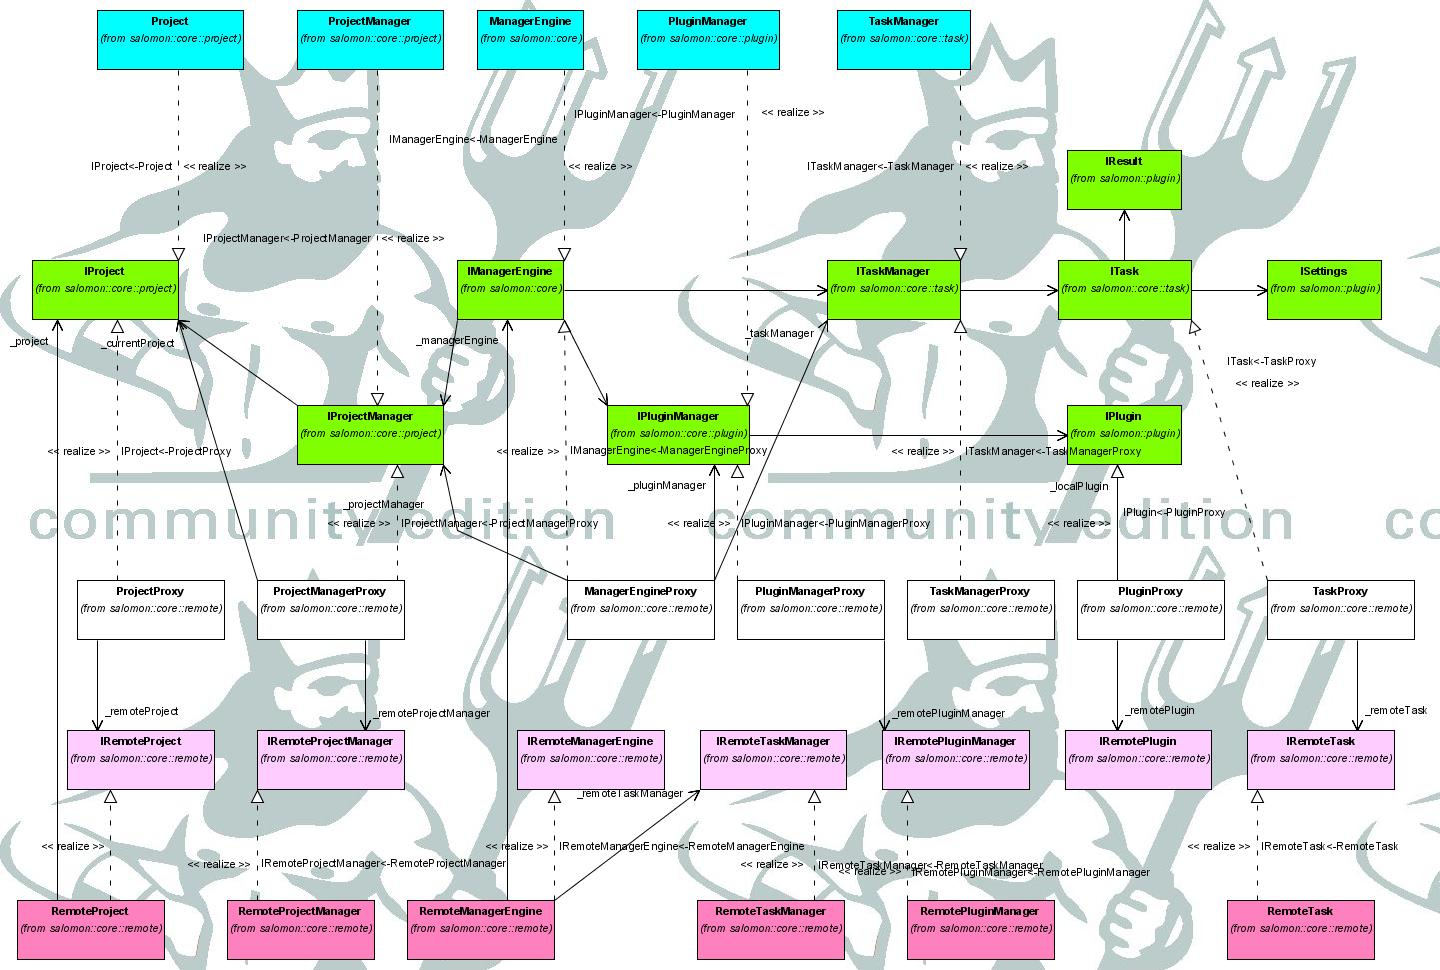
\includegraphics[scale=0.45, angle=270]{img/uml/communication.jpg}
	\caption{Warstwowa struktura klas}
	\label{fig:Communication}
\end{figure}

%\section{Dzia�anie systemu}

\subsection{Przypadki u�ycia}
Aktorem w systemie jest u�ytkownik Salomona. To on (i tylko on) jest odpowiedzialny za skonfigurowanie sobie m.in. po��czenia do bazy danych (stworzenie odpowiedniego \emph{Solution}), on te� tworzy zadania, ustala sekwencj� ich wykonywania, a nast�pnie uruchamia je i monitoruje wyniki.

\begin{figure}[h]
	\centering
		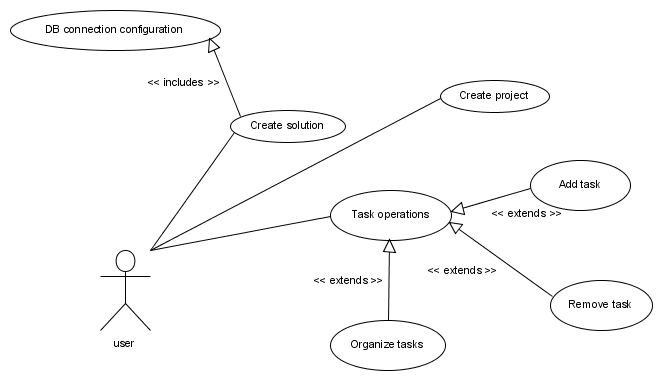
\includegraphics[width=\textwidth]{img/uml/use_case_1.png}
	\caption{Use case - operacje administracyjne: tworzenie zada�}
	\label{fig:use_case}
\end{figure}

\begin{center}
\begin{tabular}{|l|l|}
\hline  
\textbf{Use Case} & \textbf{Opis} \\
\hline  
Create Solution & Terminem tym okre�lamy struktur� \\
								& grupuj�c� kilka projekt�w. Zadanie to \\
								& wymaga konfiguracji, w szczeg�lno�ci \\ 
								& wskazania lokacji bazy danych \\
\hline  
Create Project & Stworzenie projektu  \\
\hline 
Add Task & Akcja dodania nowego zadania polega na \\
										& wstawieniu do kolejki zada� do wykonania,\\
										& pluginu implementuj�cego funkcjonalno�� tego\\
										& zadania. Dodatkowo okre�lamy nast�puj�ce po \\
										& nim zadnie oraz zadanie poprzedzaj�ce, oraz \\
										& dokonujemy edycji ustawie� zadania. \\
\hline 
Remove Task & Akcja usuwa aktualnie zaznaczone zadnie. \\
\hline  
Organize Tasks & Organizowanie zada� \\
												 & Ustawianie poprzednik�w, nast�pnik�w \\
            						 & Pozwala na zmian� aktualnej kolejno�ci \\
            						 & wykonywania zada�. \\
\hline  
DB connection configuration & Konfiguracja Bazy danych \\
\hline  												 
\end{tabular}  
\end{center}






\begin{figure}[h]
	\centering
		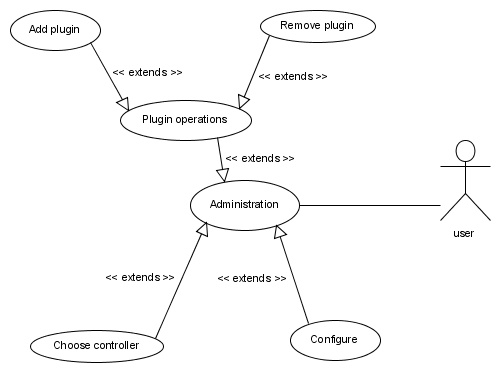
\includegraphics[width=\textwidth]{img/uml/use_case_2.png}
	\caption{Use case - operacje administracyjne: operacje na pluginach}
	\label{fig:use_case}
\end{figure}
\begin{center}
\begin{tabular}{|l|l|}
\hline  
\textbf{Use Case} & \textbf{Opis} \\
\hline  
Configure & Konfiguracja pozwala nam dostosowa� system \\
												 & do w�asnych potrzeb, podczas tego kroku \\
												 & mo�emy wyspecyfikowa� wszystkie parametry pracy \\
												 & systemu jako ca�o�ci, czyli parametry takie jak \\
												 & lokalizacja bazy danych b�d� rozproszenie systemu.  \\
\hline  
Choose controller & Wybranie rodzaju kontrolera \\
																 & Pozwala ustali� jak� funkcj� ma pe�ni� Salomon \\
																 & tj. Czy ma pe�ni� rol� Serwera, Klienta czy \\
																 & mo�e ma pracowa� sam. \\
\hline  
Add plugin & Dodanie Pluginu \\
\hline  
Remove plugin & Usuni�cie pluginu \\
\hline  												 
\end{tabular}  
\end{center}





\begin{figure}[h]
	\centering
		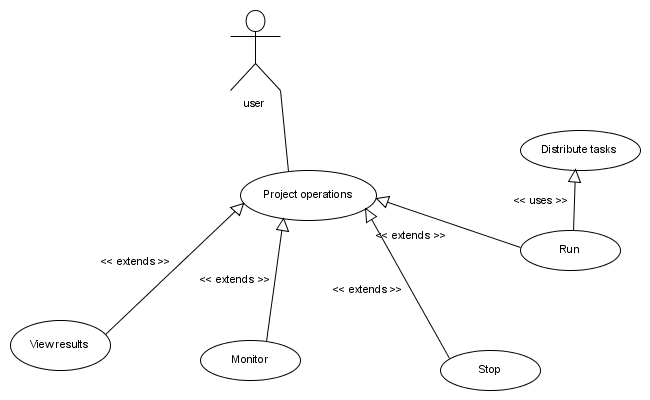
\includegraphics[width=\textwidth]{img/uml/use_case_3.png}
	\caption{Use case: operacje na projekcie}
	\label{fig:use_case}
\end{figure}

\begin{center}
\begin{tabular}{|l|l|}
\hline  
\textbf{Use Case} & \textbf{Opis} \\
\hline 
Run & Akcja ta powoduje wykonanie zada� zgromadzonych\\
											 & w tym projekcie. Wykonanie tej akcji wymaga wcze�niejszej\\
											 & konfiguracji w postaci specyfikacji listy zada� do \\
											 & wykonania oraz ich indywidualnej konfiguracji.  \\
\hline  
Stop & Przerywa aktualnie wykonywana list� zada�. \\
												& Je�li aktualnie wykonywane jest zadnie, to czy \\
												& je przerwa� le�y w gestii u�ytkownika. Je�li \\
												& dokona on wyboru, �e zadanie ma by� przerwane \\
												& natychmiast, wyniki z poprzedniego zadnia nie \\
												& ulegaj� zmianie, w przeciwnym wypadku projekt \\ 
												& zostaje zako�czony po zako�czeniu bie��cego zadnia \\
\hline  											
Monitor & W podstawowej wersji monitorowanie wykonania\\
													 & polega� b�dzie na wy�wietleniu progress bar'a,\\
													 & kt�rego stan b�dzie zmieniany po ka�dym wykonaniu\\
													 & zadnia atomowego. W nast�pnych wersjach mo�e \\
													 & pojawi� si� mo�liwo�� rejestracji zdarze� aktualnie \\
													 & wykonywanego zadania informuj�cych o jego stanie. \\
\hline  												 
View Results & Ka�de zadnie samo specyfikuje jak b�dzie \\
																& prezentowa� swoje wyniki, wi�c po wybraniu \\
																& tej akcji inicjatywa prezentacji wynik�w spada\\
																& na zadanie. Domy�lnie prezentowane s� wyniki \\
																& ostatniego zadnia ko�cz�cego przetwarzanie,\\
																& mo�emy jednak, podczas wykonywania projektu,\\
																& przejrze� wyniki ka�dego z zada� cz�stkowych z \\
																& osobna. \\
\hline  												 
Distribute tasks & Ka�de zadanie z projektu b�dzie dystrybuowane \\
																& pomi�dzy dost�pne hosty, w zale�no�ci \\
																& od ich obci��enia\\
\hline  												 
\end{tabular}  
\end{center}

\subsection{Diagramy sekwencji}
\subsubsection{Dodaj zadanie}
                \begin{figure}[h]
                \centering
                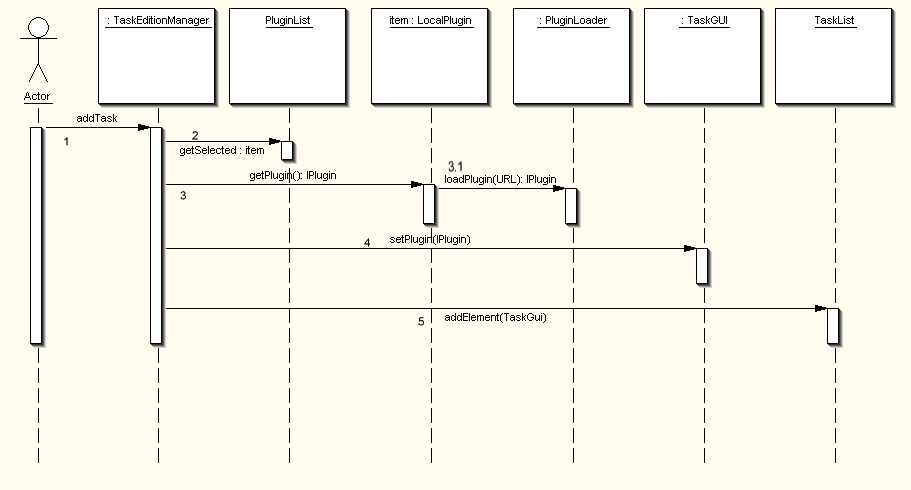
\includegraphics[width=\textwidth]{img/uml/addseq.png}
                \caption{Diagram sekwencji dla przypadku: dodaj zadanie}
                \label{fig:singleton}
                \end{figure}

\begin{enumerate}
	\item Wybieramy opcj� "`Dodaj zadanie"'
	\item Z listy dost�pnych plugin�w wybieramy jeden
	\item Plugin zostaje za�adowany
	\item Przypisujemy plugin do taska
	\item Dodajemy task do listy
\end{enumerate}
                
                
                
\subsubsection{Uruchom zadanie}                
                \begin{figure}[h]
                \centering
                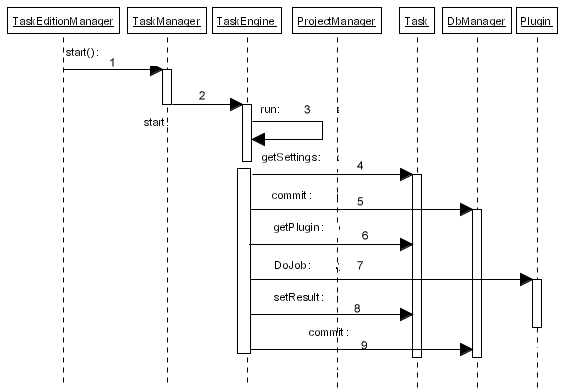
\includegraphics[width=\textwidth]{img/uml/runTaskseq.png}
                \caption{Diagram sekwencji dla przypadku: uruchom zadanie}
                \label{fig:singleton}
                \end{figure}

\begin{enumerate}
	\item Wybieramy opcj�: "`Uruchom zadanie"'
	\item TaskManager wysy�a do TaskEngine'u rozkaz uruchomienia zadania
	\item Pobranie ustawie� dla zadania
	\item Task dostaje ustawienia startowe
	\item Pobieramy plugin, kt�ry ma wykona� zadanie
	\item Wykonujemy zadanie
	\item Pobieramy wynik wykonania zadania
	\item Wysy�amy wynik do odbiorcy
\end{enumerate}

\newpage

\section{Opis bazy danych}

W systemie bardzo wa�n� rol� odgrywaj� baza danych
w kt�rej przechowywane s� ustawienia, projekty, regu�y itp.
Poni�sza struktura dotyczy tylko organizacji danych wykorzystywanych do przetwarzania wiedzy. 
Rzeczywiste dane, na podstawie kt�rych wiedza ta jest tworzona przechowywana 
jest w osobnych bazach danych i dane te nie s� kopiowane do bazy \emph{Salomona}.

\subsection{Struktura platformy}

Dane zosta�y zorganizowane w nast�puj�cych tabelach:

\subsubsection{Solutions}

Tabela reprezentuje obiekty \emph{Solution}, kt�re grupuj� projekty dotycz�ce tej samej tematyki i operuj� na tej samej bazie danych.

\begin{itemize}
		\item \emph{solution\_id} -- identyfikator obiektu \emph{solution}
		\item \emph{solution\_name} -- nazwa		
		\item \emph{solution\_info} -- dodatkowy opis
		\item \emph{hostname} -- host, na kt�rym znajduje si� baza danych
		\item \emph{db\_path} -- �cie�ka do pliku bazy danych na serwerze
		\item \emph{username} -- nazwa u�ytkownika u�ywanego do po��czenia z baz� danych
		\item \emph{passwd} -- has�o potrzebne do zalogowania si�
		\item \emph{lm\_date} -- data ostatniej modyfikacji
\end{itemize}

\subsubsection{Projects}

Tabela zawiera nag��wki projekt�w, do kt�rych odnosz� si� rekordy
z tabeli \emph{Tasks}.

\begin{itemize}
    \item \emph{project\_id} -- identyfikator projektu
    \item \emph{solution\_id} -- powi�zanie z tabel� \emph{solutions}
    \item \emph{project\_name} -- nazwa
    \item \emph{project\_info} -- dodatkowy opis
    \item \emph{env} -- reprezentuje �rodowisko, za pomoc� kt�rego przekazywane s� ustawienia mi�dzy poszczeg�lnymi zadaniami
    \item \emph{lm\_date} -- data ostatniej modyfikacji
\end{itemize}

\subsubsection{Plugins}

Tabela zawiera informacje o pluginach, kt�re mog� by� wykorzystane
przez system. Przechowuje dane o ich nazwach i lokalizacjach, sk�d
mog� by� pobrane.

\begin{itemize}
    \item \emph{plugin\_id} -- identyfikator pluginu
    \item \emph{plugin\_name} -- nazwa pluginu
    \item \emph{plugin\_info} -- dodatkowy opis
    \item \emph{location} -- lokalizacja pluginu
    \item \emph{lm\_date} -- data ostatniej modyfikacji
\end{itemize}

\subsubsection{Tasks}

Tabela zawiera zapis wykonania poszczeg�lnych zada�. Dla ka�dego z nich
przechowywane s� informacje o pluginie, kt�ry zosta�
wykorzystany do wykonania zadania; projekcie, w ramach kt�rego
zadanie zosta�o zapisane; ustawieniach, z jakimi zosta�o wykonane;
rezultacie zadania oraz statusie, w jakim pozostaje po wykonaniu.

\begin{itemize}
    \item \emph{task\_id} -- identyfikator zadania
    \item \emph{task\_nr} -- numer zadania w kolejce do ich wykonania
    \item \emph{project\_id} -- identyfikator projektu, do kt�rego nale�y zadanie
    \item \emph{plugin\_id} -- identyfikator pluginu, kt�ry wykonywany jest w ramach tego zadania
    \item \emph{name} -- nazwa
    \item \emph{info} -- dodatkowy opis
    \item \emph{plugin\_settings} -- ustawienia pocz�tkowe pluginu
    \item \emph{plugin\_result} -- rezultat dzia�ania pluginu
    \item \emph{status} -- status wykonania zadania
\end{itemize}

    Relacje mi�dzy nimi zobrazowane s� na rysunku (Rys \ref{fig:database})

\begin{figure}[H]
	\centering
		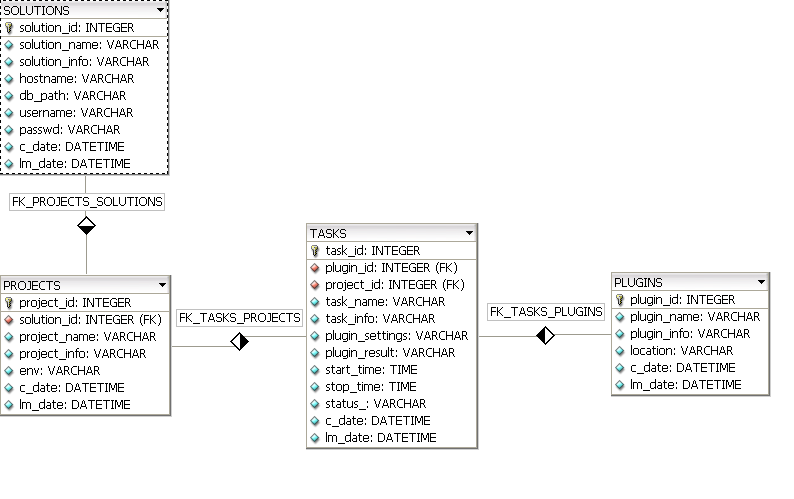
\includegraphics[width=0.90\textwidth]{img/salomon/concept/salomon_db.png}
	\caption{Relacje mi�dzy tabelami platformy}
	\label{fig:database}
\end{figure}

\subsection{Organizacja wiedzy}

\emph{Salomon} wspiera kilka rodzaj�w wiedzy: zbiory danych (\emph{datasets}),
atrybuty oraz drzewa decyzyjne.

\subsubsection{Datasets}

Tabela zawiera nag��wki zbior�w danych.

\begin{itemize}
    \item \emph{dataset\_id} -- identyfikator zbioru danych
    \item \emph{solution\_id} -- powi�zanie z tabel� \emph{solutions}
    \item \emph{dataset\_name} -- nazwa
    \item \emph{dataset\_info} -- dodatkowy opis
    \item \emph{lm\_date} -- data ostatniej modyfikacji
\end{itemize}

\subsubsection{Dataset\_items}

Zawiera definicje zbior�w zada�. Zbi�r danych definiowany jest
przez nazw� tabeli oraz warunki, jakie ograniczaj� rekordy w tej
tabeli. Tabela ta s�u�y do przechowywania podzbioru danych pochodz�cych z rzeczywistej bazy danych.

\begin{itemize}
    \item \emph{dataset\_item\_id} -- identyfikator elementu zbioru danych
    \item \emph{dataset\_id} -- identyfikator zbioru danych, do kt�rego nale�y
element
    \item \emph{table\_name} -- nazwa tabeli
    \item \emph{condition} -- warunek ograniczaj�cy zakres danych
\end{itemize}

\subsubsection{Attributesets}

Tabela zawiera nag��wki zbior�w atrybut�w.

\begin{itemize}
    \item \emph{attributeset\_id} -- identyfikator zbioru atrybut�w
    \item \emph{solution\_id} -- powi�zanie z tabel� \emph{solutions}
    \item \emph{attributeset\_name} -- nazwa
    \item \emph{attributeset\_info} -- dodatkowy opis
    \item \emph{lm\_date} -- data ostatniej modyfikacji
\end{itemize}

\subsubsection{Attributeset\_items}

Tabela przechowuje atrybuty, nale��ce do danego zbioru atrybut�w.
Ka�dy atrybut ma nazw� oraz typ. Obecnie wspierane s� atrybuty typu tekstowego,
numeryczne (ca�kowite i zmiennoprzecinkowe) oraz wyliczeniowe.
Dla atrybut�w typu wyliczeniowego, w polu $attribute_value$ przechowywana jest
lista warto�ci, kt�re dany atrybut mo�e przyjmowa�.
Atrybuty odpowiadaj� kolumnom z bazy danych, st�d ka�dy z nich przechowuje
odwolanie do kolumny w tabeli, na podstawie kt�rej zosta� zdefiniowany. 

\begin{itemize}
  	\item \emph{attributeset\_item\_id} -- identyfikator atrybutu
    \item \emph{attributeset\_id} -- identyfikator zbioru atrybut�w, do kt�rego
    dany atrybut nale�y
    \item \emph{solution\_id} -- powi�zanie z tabel� \emph{solutions}
    \item \emph{attribute\_name} -- nazwa
    \item \emph{attribute\_type} -- typ atrybutu
	\item \emph{table\_name} -- nazwa tabeli, na podstawie kt�rej atrybut zosta�
	zdefiniowany
	\item  \emph{column\_name} -- nazwa kolumny z tej tabeli
	\item  \emph{attribute\_value} -- lista warto�ci, kt�re atrybut mo�e
	przyjmowa�. Dotyczy atrybut�w typu wyliczeniowego.
\end{itemize}

\subsubsection{Trees}

Tabela przechowuje nag��wki drzew decyzyjnych. Zawiera odniesienie do zbioru
atrybut�w, gdy� to w�a�nie na ich podstawie drzewa s� budowane.

\begin{itemize}
  	\item \emph{tree\_id} -- identyfikator drzewa decyzyjnego
    \item \emph{attributeset\_id} -- identyfikator zbioru atrybut�w
    \item \emph{solution\_id} -- powi�zanie z tabel� \emph{solutions}
    \item \emph{root\_node\_id} -- identyfikator korzenia drzewa
    \item \emph{tree\_name} -- nazwa
    \item \emph{tree\_info} -- dodatkowy opis
    \item \emph{lm\_date} -- data ostatniej modyfikacji
\end{itemize}

\subsubsection{Tree\_nodes}

Zawiera definicje w�z��w drzewa decyzyjnego.

\begin{itemize}
  	\item \emph{node\_id} -- identyfikator w�z�a
  	\item \emph{tree\_id} -- identyfikator drzewa decyzyjnego, do kt�rego nale�y
    \item \emph{parent\_node\_id} -- identyfikator w�z�a rodzica (0 dla korzenia)
    \item \emph{attribute\_item\_id} -- identyfikator atrybutu, kt�remu w�ze� odpowiada
    \item \emph{parent\_edge\_value} -- warunek na kraw�dzi prowadz�cej do w�z�a
    \item \emph{node\_value} -- warto�� w w�le
\end{itemize}





\section{Wtyczki}

System, dzi�ki swej elastycznej architekturze, pozwala u�ytkownikowi na 
rozszerzanie jego mo�liwo�ci poprzez definiowanie przez niego w�asnych 
wtyczek. Dzi�ki takiemu podej�ciu system jest �atwo skalowalny
i rozszerzalny o~nowe mo�liwo�ci. 

Ca�a funkcjonalno�� zwi�zana z~konfiguracj�  przetwarzaniem, prezentacj� wynik�w dzia�ania oraz komunikacj� przez sie� ukryta jest przed tw�rc� wtyczki i~nie musi by� brana pod uwag� przy jego projektowaniu i~implementacji. Jedyne, co musi on zrobi� to~zaimplementowa� opisane poni�ej interfejsy.
By system m�g� skorzysta� z~nowych wtyczek nale�y 
poda� ich lokalizacje, umo�liwiaj�c systemowi tym samym pobranie i~
za�adowanie wtyczki. Obecna wersja systemu obs�uguje tylko wtyczki w~postaci 
archiw�w jar.

Poni�y diagram (Rys. \ref{fig:plugin_uml}) przedstawia podstawowe interfejsy
potrzebne do implementacji w�asnej wtyczki. Kolorem ��tym zaznaczone
zosta�y interfejsy zwi�zane z~graficzn� cz�ci� wtyczki. Kolorem niebieskim
interfejs, kt�ry zwi�zany jest z~algorytmem wtyczki. 

\begin{figure}[H]
	\centering
		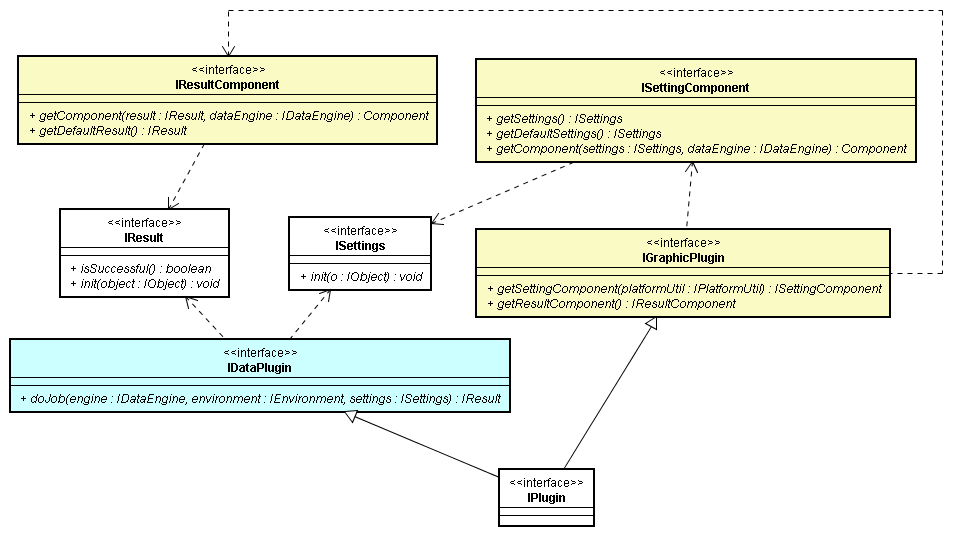
\includegraphics[width=0.90\textwidth]{img/salomon/uml/plugin.png}
	\caption{Interfejsy wtyczki}
	\label{fig:plugin_uml}
\end{figure}

\subsection{IPlugin}

Jest to~g��wny interfejs implementowany przez wszystkie wtyczki. Stanowi po��czenie interfejs�w \emph{IDataPlugin}~(\ref{lab:data_plugin}) i~\emph{IGraphicPlugin}~(\ref{lab:graphic_plugin}).
 
\subsection{IDataPlugin}
\label{lab:data_plugin}

Interfejs ten definiuje tylko jedn� metod� \emph{doJob()}, kt�ra jest uruchamiana podczas przetwarzania danej wtyczki i~stanowi jej g��wne zadanie obliczeniowe. Jej parametry to:

\begin{itemize}
	\item \emph{IDataEngin}~(\ref{lab:data_engine}) -- obiekt ten dostarcza interfejs�w pozwalaj�cych na operowanie na danych i~wiedzy (np. ITreeManager)
 	\item \emph{IEnvironment} to~interfejs umo�liwiaj�cy komunikacje 
          pomi�dzy poszczeg�lnymi zadaniami
	\item \emph{ISettings} reprezentuj� konfiguracja wej�ciowa wtyczki
\end{itemize}  
    
\subsection{IGraphicPlugin}
\label{lab:graphic_plugin}
Interfejs ten okre�la spos�b, w~jaki wtyczka mo�e by� konfigurowana przez u�ytkownika oraz jak maj� by� prezentowane wyniki oblicze�. 
\begin{itemize}
	\item \emph{getSettingComponent()} -- zwraca obiekt implementuj�cy interfejs 
		\emph{ISettingComponent}~(\ref{lab:setting_component})
	\item \emph{getResultComponent()} -- zwraca obiekt implementuj�cy interfejs 
		\emph{IResultComponent}~(\ref{lab:result_component})
\end{itemize}

\subsection{ISettingComponent}
\label{lab:setting_component}
\begin{itemize}
	\item \emph{getComponent(ISettings settings)} -- zwraca graficzny komponent 
s�u��cy do edycji ustawie� wtyczki. Jest on wype�niany warto�ciami przekazanymi 
w obiekcie \emph{ISettings}.
	\item \emph{getSettings()} -- zwraca ustawienia wtyczki.
	\item \emph{getDefaultSettings()} -- zwraca domy�lne ustawienia wtyczki. 
Wykorzystywane, gdy u�ytkownik nie wprowadzi� w�asnych ustawie�.
\end{itemize}    

\subsection{IResultComponent}
\label{lab:result_component}
\begin{itemize}
	\item \emph{getComponent(IResult result)} -- zwraca graficzny komponent 
wy�wietlaj�cy rezultat wykonania wtyczki. Wype�niany jest on na podstawie 
obiektu  \emph{IResult} zwr�conego wcze�niej przez metod� \emph{doJob()}.
	\item  \emph{getDefaultResult()} -- zwraca domy�lny rezultat wykonania wtyczki.
\end{itemize}

\subsection{IObject} To~interfejs zapewniaj�cy persystencj� takich obiekt�w 
jak ustawienia, rezultat wykonania wtyczki, czy obiekty wykorzystywane do komunikacji mi�dzy wtyczkami.

\subsection{ISettings}Implementowany przez obiekt reprezentuj�cy ustawienia 
wtyczki.
\begin{itemize}
	\item \emph{init(IObject o)} - metoda inicjalizuje obiekt klasy
\end{itemize}    

\subsection{IResult} Implementowany przez obiekt reprezentuj�cy rezultat 
dzia�ania wtyczki.
\begin{itemize}
	\item \emph{init(IObject o)} - metoda inicjalizuje obiekt klasy
\end{itemize}  

%WSTAWI� TO W~JAKIE� MIEJSCE!!!
%
%\paragraph{Persystencja danych}
%Z racji na rozproszony charakter aplikacji, oraz na wielko�� oblicze�.
%Wa�nym aspektem platformy jest zapewnienie uniwersalnego i~wydajnego
%mechanizmu persyste�cji danych. W~przypadku wewn�trznych struktur danych,
%jak zapis drzewa decyzyjnego, czy atrybut�w, zadaniem tym zajmuj� si�
%odpowiednie menadz�ry. W~przypadku jednak persystencji danych u�ytkownika,
%takich jak ustawienia wtyczek, czy ich rezultaty zadaniem tym zajmuj� si�
%modu� persyste�cji, udost�pniaj�cy odpowiedni \emph{API}. Dodatkowo mechanizm
%ten jest wykorzystywany do persystencji danych wykorzystywanych w~komunikacji mi�dzy kolejnymi zadaniami (WSTAWI� LINKA DO OPISU ENV.)
%
%Kod poni�ej tworzy struktur�, z~jednym polem o~nazwie ,,myField'' oraz przypisuje do niego warto�� ,,my settings''.
%
%\begin{lstlisting}
%SimpleStruct struct = new SimpleStruct();
%struct.setField("myField", "my settings");
%\end{lstlisting}
%
%WSTAWI� UML? 



\section{Uruchomienie}
Do uruchomienia programu konieczne jest zainstalowanie w systemie \emph{Java Runtime Environment} , w wersji 1.5. Je�li program ma dzia�a� z wykorzystaniem niezale�nego serwera bazy danych \emph{Firebird}, to nale�y zainstalowa� dodatkowo baz� \emph{Firebird}.

Program mo�e dzia�a� w 3 trybach (jako serwer, klient lub lokalnie) i na dwa sposoby ��czy� si� z baz� danych (poprzez serwer lub bez niego), zale�nie od wpis�w w pliku konfiguracyjnym. 
Aby uruchomi� go w odpowiedniej konfiguracji, nale�y rozpakowa� go i zmodyfikowa� domy�lne ustawienia pliku konfiguracyjnego. Program dostarczany jest z przyk�adow� baz� danych w kt�rej zdefiniowane s� odpowiednie tabele i lokalizacje plugin�w oraz z przyk�adowymi pluginami. 
Dla u�ytkownik�w, kt�rzy chc� stworzy� w�asn� baz� danych w katalogu db umieszczony zosta� skrypt, tworz�cy tabele niezb�dne do pracy programu i uruchomienia dostarczonych plugin�w (crebas.sql).

\subsection{Plik konfiguracyjny}
G��wnym plikiem konfiguracyjnym programu jest config.properties.
Zawiera on nast�puj�ce klucze:

\begin{itemize}
\item \emph{HOSTNAME} - identyfikator sieciowy komputera, na kt�rym zainstalowana jest baza danych. Uwzgl�dniany jest tylko w przypadku, gdy program ��czy si� z baz� danych przy u�yciu serwera Firebird.

\item \emph{DB\_PATH} - lokalizacja bazy danych. Gdy program dzia�a z serwerem Firebird jest to lokalizacja bezwzgl�dna, w przeciwnym przypadku - wzgl�dem katalogu instalacyjnego.

\item \emph{USER} - nazwa u�ytkownika, kt�ry loguje si� do bazy

\item \emph{PASSWD} - has�o u�ytkownika

\item \emph{EMBEDDED} - okre�la, spos�b po��czenia z baz� danych
\subitem \emph{N} - z wykorzystaniem serwera
\subitem \emph{Y} - przy u�yciu dll-a

\item \emph{SERVER\_HOST} - nazwa komputera, na kt�rym zainstalowany jest Salomon w wersji server

\item \emph{SERVER\_PORT} - port na kt�rym nas�uchuje server

\item \emph{MODE - tryb} uruchomienia
\subitem \emph{local} - lokalnie
\subitem \emph{client} - klient
\subitem \emph{server} - serwer

\end{itemize}

Pozosta�e warto�ci nie powinny by� modyfikowane przez u�ytkownika.

\subsection{Ustawienia pliku konfiguracyjnego}
\paragraph{Tryb serwera}
\begin{itemize}
    \item \emph{MODE=server}
    \item \emph{SERVER\_HOST=IP hosta}
    \item \emph{SERVER\_PORT=nr portu}
\end{itemize}

\paragraph{Tryb klienta}
\begin{itemize}
    \item \emph{MODE=server}
    \item \emph{SERVER\_HOST=IP sewera}
    \item \emph{SERVER\_PORT=nr portu na kt�rym nas�uchuje serwer}
\end{itemize}

\paragraph{Tryb lokalny}
\begin{itemize}
    \item \emph{MODE=local}
\end{itemize}

We wszystkich trybach mo�liwe jest ustawienie po��czenie z baz� danych za pomoc� serwera Firebird lub przy u�yciu dll-a (klucz \emph{EMBEDDED}).

\section{Interfejs u�ytkownika}

\subsection{Tryb serwera}
G��wnym zadaniem systemu jest umo�liwienie definiowania i wykonywania zada� w oparciu o dost�pne pluginy. Gdy program dzia�a w trybie serwera po lewej stronie widoczna jest lista pod��czonych klient�w. Wszystkie opisane poni�ej operacje wykonywane s� dla aktualnie wybranego klienta.

\subsubsection{Zadania}
Aby zdefiniowa� nowe zadanie, nale�y wybra� plugin, za pomoc� kt�rego b�dzie ono realizowane oraz skonfigurowa� jego ustawienia. Plugin nale�y wybra� z listy dost�pnych plugin�w, znajduj�cej si� na �rodku g��wnego okna programu. Po wybraniu pluginu i naci�ni�ciu przycisku ze strza�k� w prawo znajduj�cego si� miedzy panelem z pluginami a panelem z zadaniami pojawia si� okienko, w kt�rym nale�y wprowadzi� nazw� zadania. 


%\paragraph{@@@PIPCZER}
\paragraph{}

Po potwierdzeniu nazwy zostanie utworzone nowe zadanie i dodane do listy zada�. Ka�de z zada� mo�na skonfigurowa� przed wykonaniem, w tym celu nale�y nad wybranym zadaniem wywo�a� menu kontekstowe (prawym klawiszem myszy) i wybra� opcj� \textbf{Settings}. Po jej wybraniu pojawi si� okienko s�u��ce do konfiguracji zadania - mo�e by� r�ne, zale�nie od pluginu kt�ry ma by� wykonany w ramach zadania. 

%\paragraph{@@@PIPCZER}


\paragraph{}
Po skonfigurowaniu zada� nale�y zatwierdzi� list� zada� do wykonania za pomoc� klawisza \textbf{Apply}. Je�li zadania nie zosta�y wcze�niej zapisane w ramach projektu, pojawi si� okienko w kt�rym nale�y poda� nazw� projektu. Po poprawnym zapisaniu projektu mo�na wykona� zaplanowane zadania. Zostan� one wykonane  w takiej kolejno�ci, w jakiej znajduj� si� one na li�cie zada�. Mo�liwa jest zmiana tej kolejno�ci - s�u�� do tego przyciski ze strza�kami znajduj�ce si� po prawej stronie panelu z zadaniami. Je�li zostanie ustalona ostateczna kolejno�� zada�, mo�na je wykona� za pomoc� przycisku Run.

\paragraph{}
Po wykonaniu zada� mo�na obejrze� ich rezultaty. W tym celu nale�y z menu kontekstowego dla zada� wybra� opcj� \textbf{Result}. Po jej wybraniu pojawi si� okienko prezentuj�ce wyniki wykonania danego zadania. Jego wygl�d, podobnie jak w przypadku ustawie� zada�, zale�y od pluginu.

\subsubsection{Pluginy}
Lista plugin�w tworzona jest na podstawie odpowiednich wpis�w w bazie danych. Mo�na j� jednak  modyfikowa� - dodawa�, usuwa� lub modyfikowa� dane pluginy. S�u�� do tego odpowiednie opcje z menu kontekstowego wywo�ywanego dla plugin�w. 

%\paragraph{@@@PIPCZER}


\subsubsection{Projekty}

Konfiguracja plugin�w oraz lista zada� zapisywana jest w ramach projekt�w. Dzi�ki temu mo�na zdefiniowa� r�ne listy zada� i wykonywa� je wielokrotnie, bez potrzeby ich ponownego tworzenia i konfiguracji. Aby za��dowa� istniej�cy projekt nale�y z menu g��wnego wybra� pozycj� \textbf{Projects$\rightarrow$Open Project}. Spowoduje to wy�wietlenie listy zapisanych projekt�w i umo�liwi wyb�r projektu do za�adowania. 

\subsection{Tryb klienta}
Program pracuj�cy w tym trybie nie posiada interfejsu u�ytkownika, jego konfiguracja odbywa si� z serwera.

\subsection{Tryb lokalny}
Interfejs dla programu dzia�aj�cego w trybie lokalnym zbli�ony jest do programu w trybie serwera. Nie posiada on jednak listy pod��czonych klient�w, gdy� sam wykonuje zdefiniowane zadania, czyli zachowuje si� jak po��czenie dw�ch program�w dzia�aj�cych w trybie serwera i klienta.

\subsection{SQL Console}
W trybie serwera oraz w trybie lokalnym z menu Tools dost�pny jest program SQL Console. Pozwala on na wykonywanie zapyta� SQL-owych, przez co umo�liwia administracj� projektami, pluginami i zadaniami oraz innymi tabelami wykorzystywanymi przez system.


\section{Za�o�enie implementacyjne}
W czasie produkcji systemu stosowali�my nast�puj�ce zasady:

\subsection{Kontrola wersji}
Ca�y kod oraz inne zasoby wykorzystywane w programie znajduj� si� pod kontrol� wersji. U�ywany do tego jest  \emph{Subversion} (nast�pca CVS-a) i odpowiednie pluginy zapewniaj�ce jego integracj� z edytorem oraz systemem operacyjnym. Zapewnia to pe�n� synchronizacj� kodu na wszystkich komputerach, na kt�rych mo�e on by� modyfikowany.

\subsection{Wsp�lny edytor}
U�ywany jest wsp�lny edytor - \emph{Eclipse}. Dzi�ki mo�liwo�ci eksportowania ustawie� u�ywane jest  identyczne formatowanie kodu, co pomaga utrzyma� przejrzysto�� i czytelno�� kodu. 

\subsection{Testowanie jednostkowe} 
W celu testowania funkcjonalno�ci wykorzystujemy mechanizm \emph{JUnit}. 

\subsection{GUI testowanie}
W celu weryfikowania poprawno�ci interfejsu u�ytkownika stworzone zosta�y skrypty dla programu Abbot. Jego zadaniem jest odtworzenie nagranych sekwencji wykonywanych  przez  u�ytkownika w czasie obs�ugi programu. W po��czeniu z runtime-ow� weryfikacj� kontrakt�w stanowi to silny mechanizm weryfikacji jako�ci produktu

\subsection{Kontrakty}
W kodzie zosta�y wprowadzone mechanizmy zaczerpni�te z j�zyka  \emph{Eiffel} - tzw. kontrakty. Polega to na tym, �e w komentarzach dla klas oraz metod zawarte s� warunki, sprawdzaj�ce poprawno�� stanu, w jakim znajduje si� system. Kontrakty stanowi� dodatkow� informacj� dla programisty wykorzystuj�cego dan� klas� lub interfejs. Dodatkowo wykorzystywany jest kompilator, kt�ry kompiluje tak�e kod kontrakt�w i w razie ich z�amania rzuca wyj�tki.

\subsection{Automatyczne budowanie projektu} 
W celu zautomatyzowania procesu budowania projektu wykorzystany zosta� program  \emph{Ant}. Automatyzuje on proces tworzenia projektu od kompilacji, a� do wygenerowania instalatora.

\subsection{Instalator}
By upro�ci� proces instalacji dla u�ytkownika ko�cowego utworzone zosta�y skrypty tworz�ce instalator. Jako program do utworzenia instalatora wykorzystywany jest program  \emph{IzPack}.

\subsection{Mechanizmy lokalizacyjne}
Wszystkie teksty u�yte w interfejsie u�ytkownika pobierane s� z odpowiednich plik�w, co pozwala na �atw� lokalizacj� programu

\subsection{Konfiguracja}
Konfiguracja programu wczytywana jest z odpowiednich plik�w konfiguracyjnych. Pozwala to na �atw� zmian� zachowania programu (np. zmian� kontrolera). 

\subsection{Logowanie}
Do �ledzenia przebiegu wykonania programu wykorzystywany jest log4j. Wprowadza on elastyczny model logowania. 

\subsection{Zarz�dzanie projektem}
Jak system zarz�dzania projektem wybrali�my Gemini - system wspomagania pracy grupowej oparty na ASP.NET. System wspomaga wszelkie dziedziny �ycia projektu, poczynaj�c od przydzia�u zada� dla poszczeg�lnych developer�w, kontroli stanu ich wykonania, estymacji czasu pracy nad danym zagadnieniem, po zarz�dzanie projektem jak ca�o�ci� czyli wyznaczanie milestone'�w oraz przypisywania do nich zada�, generacja diagram�w Gantta, zarz�dzanie zasobami ludzkimi itp. 

%\subsection{CMS}
%Jako CMS(Content Management System) dla naszej strony zosta� u�yty projekt Mambo 4.9.1a. Jest to bardzo wygodny i %elastyczny w u�ytkowaniu system kontroli tre�ci. System ma budow� modu�ow� dzi�ki czemu mo�emy w ka�dej chwili rozszerzy� %jego funkcjonalo��. Opr�cz standardowych modu��w jakie dostarczane s� z dystrybucj� Mambo do��czyli�my Forum dyskusyjne %(SimpleBoard) oraz galeri� (RSGallery). Dodatkow� mo�liwo�ci� jest wrappowanie innych projekt�w dzi�ki czemu uda�o nam %sie bez wi�kszych problem�w doda� modu�y bezpo�rednio nie wspierane przez Mambo, jak Bugzilla czy Wiki.


%\subsection{Maven}
%W projekcie u�yli�my r�wnie� mavena. Jest to bardzo u�yteczne narz�dzie do zarz�dzania buildami, jak r�wnie� tworzeniem raport�w na temat posuwaj�cych si� prac. Aktualnie podpi�li�my nast�puj�ce raporty:
%\begin{itemize}
%	\item Changes\\
%	w estetyczny spos�b pokazuje wersje, i zmiany jakie w nich zasz�y
%	\item Checkstyle\\
%	raport z checkstyle'a \href{http://checkstyle.sourceforge.net/}{http://checkstyle.sourceforge.net/}, najpopularniejszego chyba darmowego narz�dzia do statycznej analizy kodu)
%	\item Unit tests\\
%	Raport z przebiegu test�w wykonanych za pomoc� JUnita
%	\item File activity\\
%	Pokazuje jak cz�sto zmienia�y si� poszczeg�lne pliki
%	\item Change log\\
%	Pokazuje komentarze z wszystkich commit�w do repozytorium
%	\item PMD report\\
%	to narz�dzie(\href{http://pmd.sourceforge.net/}{http://pmd.sourceforge.net/}) wykrywa potencjalne b��dy, takie jak:
	
%		\begin{itemize}
%			\item puste bloki try/catch/finally/switch
%			\item nieu�ywane lokalne zmienne, parametry i metody prywatne
%			\item puste warunki: if/while
%		\end{itemize}
%	\item Javadocs
%	\item Kod w postaci plik�w html
%\end{itemize}
%\section{Testy}
\subsection{JUnit}

\subsubsection*{Wrappery na obiekty}
${salomon.engine.serialization.IObjectComparatorTest}$\\
\begin{enumerate}
	\item testCompareInt()\\
	Tworzy dwie klasy \texttt{SimpleInteger}(implementacja \texttt{IInteger}) i inicjuje je tymi samymi warto�ciami. Nast�pnie wykonywany jest
	
\begin{verbatim}
assertTrue(int1.equals(int2));
\end{verbatim}
Tworzymy te� 3 obiekt, kt�ry inicjujemy inn� warto�ci� i wykonujemy:
\begin{verbatim}
assertFalse(int1.equals(int3));
\end{verbatim}

	\item testCompareString()\\
	Analogiczny test, tyle �e dla obiekt�w 	\texttt{SimpleString}(implementacja \texttt{IString})

	\item testCompareStuct()\\
	Analogiczny test, tyle �e dla obiekt�w 	\texttt{SimpleStruct}(implementacja \texttt{IStruct})

\end{enumerate}

\subsubsection*{Klasy rdzenia}
${salomon.engine.solution.SolutionManagerTest}$\\
Test obejmuje wszystkie dzia�ania na "`Rozwi�zaniach"' takie jak tworzenie samego Rozwi�zania oraz dodanie do niego poszczeg�lnych projekt�w, testowane jest r�wnie� przechowywanie rozwi�za� w bazie danych i pobieranie ich do uruchomienia.
Funkcjonalno�� jest nowa wi�c test b�dzie sie rozrasta� w miar� jej rozbudowywania 
\begin{enumerate}
	\item testCreateSolution()\\
		Test tworzenia "`Rozwi�za�"'
	\item testGetAddSolution()\\
		Test dodaje kilka rozwi�za� do SolutionManagera oraz pr�buje je pogra� jako list�
	\item testGetSolution()\\
	  Analogiczny test do poprzedniego lecz tym razem pobieramy Rozwi�zanie o konkretnej nazwie  
\end{enumerate}


\textbf{Solution Test}\\
${salomon.engine.solution.SolutionTest}$\\
Testuje dost�pne narazie funkcjonalno�� "`Rozwi�zania"'. Jako �e rozwi�zanie jest tworzone przez SolutionManagera przetestowanego powy�ej, test sprowadza sie do wyci�gania informacji ze stworzonego rozwi�zania
Funkcjonalno�� jest nowa, wi�c test b�dzie sie rozrasta� w miar� dodawania nowej funkcjonalno�ci 


\textbf{Test Mened�era Zada�}
${salomon.engine.solution.TaskManagerTest}$\\
Testowana jest tutaj funkcjonalno�� zwi�zana z zarz�dzaniem zadaniami. Test obejmuje kompleksowe tworzenie Zadania do wykonania, dodawanie zada� do wykonania/usuwania, dodawania zada� do projektu itd. 
\begin{enumerate}
\item testCreateTask\\
			Testuje tworzenie zada� 
\item testAddTask\\
			Test dodawania/pobierania zada� do wykonania, jako �e zadania s� przechowywane w bazie danych test obejmuje g��wne funkcjonowanie bazy
\item testClearTasks\\
			Test usuwania zada� z bazy
\item testGetCurrentTask\\
			Pobiera aktualnie wykonywane zadanie
\item testSetProjectManager\\
			Testuje ustawienia projektu do wykonania
\end{enumerate}

\textbf{Test Pojedynczego zadania}
${salomon.engine.solution.TaskTest}$\\
Analogiczny do poprzedniego zestawu test�w lecz skupia si� bardziej na operowaniu samym zadaniem nie ich zbiorem

\textbf{Test Mened�era projekt�w}
${salomon.engine.project.ProjectManagerTest}$\\
Testy analogiczne do SolutionManagera, dodawanie/usuwanie projekt�w do Managera, zachowywanie projekt�w do bazy itd.

\textbf{Test Pojedynczego projektu}
${salomon.engine.project.ProjectTest}$\\
Testy operuj�ce na samum projekcie g��wnie �adowanie, zachowywanie, usuwanie projekt�w 

\subsubsection*{Baza Danych}
Ca�a komunikacja z baz� danych zosta�a owrappowana w klasy odpowiadaj�ce odpowiednim zapytaniom , testy w tej sekcji s� zaprojektowane aby testowa�y ich funkcjonalno��. Ka�da klasa test�w odpowiada jednemu typowi zapyta� i zawiera po kilka test�w.\\

\textbf{Usuwanie danych z bazy}
${salomon.engine.database.queries.SQLDeleteTest}$\\
	Testy usuwania rekord�w z baz danych\\
	
\textbf{Dodawanie danych z bazy}
${salomon.engine.database.queries.SQLInsertTest}$\\
	Testy dodawania rekord�w\\
	
\textbf{Zapytania do bazy}
${salomon.engine.database.queries.SQLSelectTest}$\\
	Testy zapyta� do bazy\\
	
\textbf{Zmiana rekord�w w bazie}\\
${salomon.engine.database.queries.SQLUpdateTest}$\\
	Testy zmiany zawarto�ci rekord�w
	 
\subsubsection*{Pluginy}

\textbf{Test Mened�era plugin�w}
${salomon.engine.plugin.PluginManagerTest}$\\
	Testy funkcjonalno�ci zwi�zanej z pluginami, jak �adowanie/dodawanie/usuwanie plugin�w z systemu, operacje na pluginach\\
	
\subsubsection*{Serializacja do XMLa}
${salomon.engine.serialization.SerializerTest}$\\
Jako przyk�adowe dane wykorzystuje ona plik:

\begin{Verbatim}
<?xml version="1.0" encoding="UTF-8"?>
<!DOCTYPE struct SYSTEM "config/struct.dtd">

<struct name="str1">
  <int name="int1" value="2301"/>
  <string name="string1" value="test_val_1"/>
  <struct name="str1_2">
    <string name="string2" value="val2"/>
    <int name="int2" value="666"/>
  </struct>
</struct>
\end{Verbatim}


Test zawiera metody:
\begin{itemize}
	\item testDeserialize()\\
	Testuje serializacj� z XML do obiektu
	\item testSerialize()\\
	Testuje serializacj� z obiektu do XML
	\item testSymetric()\\
	Wykonuje serializacj� i deserializacj� i sprawdza czy dostali�my to samo.
\end{itemize}

%\subsection{Abbot}

W projekcie chcemy doda� GUI Testy. U�ywamy do tego Abbota(\href{http://abbot.sourceforge.net/}{http://abbot.sourceforge.net/}). Jest to prosty framework pozwalaj�cy na takie w�a�nie testy. Na razie zaimplementowali�my przyk�adowy test, odpalaj�cy okienko Salomona. To podstawowy test pozwalaj�cy stwierdzi� czy program dzia�a czy nie.


\subsubsection{Instalacja}
Program mo�na �ci�gn�� ze strony projektu. Razem z dystrybucj� dostajemy przyjemne GUI do tworzenia tych test�w.
Testy zapisywane s� w XMLu.\\
Nale�y ponadto doda� odpowiednie jar-y do classpath (\texttt{abbot.jar}, \texttt{xalan.jar}, \texttt{xml-apis.jar}).
\subsubsection{Test}
\begin{Verbatim}
<AWTTestScript 
  desc="Skrypt (D:\home\krzychu\dv\ks\test\abbot\salomon.xml)"
  forked="true">
  <launch 
    args="[]"
    class="salomon.engine.Starter" 
    classpath="
      salomon.jar;
      .;
      lib\mini-j2ee.jar;
      lib\log4j-1.2.8.jar;
      lib\firebirdsql.jar"
    method="main"/>
  <wait 
    args="Salomon"
    class="abbot.tester.ComponentTester"
    method="assertFrameShowing"/>
  <terminate/>
</AWTTestScript>
\end{Verbatim}
Jak wida� w te�cie tym sprawdzamy czy okienko si� pokazuje czy te� nie.

\subsubsection{Uruchomienie testu}
\begin{Verbatim}
java -cp lib/abbot.jar 
	junit.extensions.abbot.ScriptFixture test/abbot/salomon.xml
\end{Verbatim}

Po uruchomieniu tego dostajemy output:
\begin{Verbatim}
$ runabbot.bat

D:\home\krzychu\dv\ks>java -cp lib/abbot.jar 
	junit.extensions.abbot.ScriptFixture test/abbot/salomon.xml
.
Time: 38,035

OK (1 test)
\end{Verbatim}

W planach mamy bardziej zaawansowane testy w miar� jak b�dzie si� poszerza� funkcjonalno��.

%\subsection{Grinder}
W za�o�eniach projektu to nie wydajno�� mia�a decydowa� o przydatno�ci Salomona, a mo�liwo�� �atwego pisania plugin�w do rozproszonego wykonywania zada� zwi�zanych z knowledge mining. Jednak w RMI zawsze sa pewne narzuty na komunikacje. Do testowania zamierzali�my u�y� narz�dzie zwane Grinder\\
(\href{http://grinder.sourceforge.net/}{http://grinder.sourceforge.net/})

\subsubsection{grinder.properties}
\begin{verbatim}
grinder.processes=2
grinder.threads=2
grinder.runs=1

grinder.logDirectory=log
grinder.numberOfOldLogs=2

grinder.script=scripts/register.py
\end{verbatim}

\subsubsection{Skrypty uruchomieniowe}
\begin{Verbatim}
#!/bin/bash
LIB_HOME=../../lib
CP=../../lib/grinder/grinder.jar
CP=$CP\;../../bin/
for i in `ls $LIB_HOME | grep jar`
do
CP=$CP\;$LIB_HOME/$i
done
echo $CP
java -cp $CP -Djava.security.policy=../../all.policy \\
net.grinder.Console
\end{Verbatim}

\subsubsection{Skrypt testowy}
register.py
\begin{Verbatim}
from net.grinder.script.Grinder import grinder
from net.grinder.script import Test
from java.rmi.registry import LocateRegistry
from salomon.engine.platform import ManagerEngine
from salomon.engine.remote import RemoteController
from salomon.engine.remote import ICentralController;
from java.lang import System
from java.rmi import RMISecurityManager;
# Client Properties
SERVER     = "localhost"
PORT       = 4321
test1 = Test(1, "RegisterTest")
class TestRunner:
    
    # This method is called for every run.
    def __call__(self):
        System.setSecurityManager(RMISecurityManager());
        managerEngine = ManagerEngine()
        remoteController = RemoteController(managerEngine,SERVER)
        registry = LocateRegistry.getRegistry(SERVER,PORT)
        centralController = registry.lookup("CentralController")
        centralController.register(remoteController)
        if centralController is None:
            grinder.statistics.setSuccess(0)

\end{Verbatim}

\subsubsection{Skrypt testowy nr 2}
Chocia� za pomoc� Jythona mo�na zapisa� niemal ka�dy kod Javy, zdecydowali�my si� na zmian� podej�cia i trzymanie wszystkich test�w w klasach Javy - Jythona u�ywa� b�dziemy jedynie do instancjonowania tych klas. Dzi�ki temu mo�liwe jest debuggowanie test�w w razie, gdyby kt�ry� dzia�a� niezgodnie z za�o�eniem. Nowsza wersja skryptu wygl�da tak:
\begin{Verbatim}
from net.grinder.script.Grinder import grinder
from net.grinder.script import Test
from salomon.engine import TestRegister
def registerTestCase():
	case = TestRegister()
	case.test()

testRegister = Test(1, "RegisterTest").wrap(registerTestCase)

class TestRunner:
    def __call__(self):
        testRegister()

\end{Verbatim}




\subsubsection{TestCase}
Zrobili�my na razie najprostszy mo�liwy test case polegaj�cy na zarejestrowaniu i wyrejestrowaniu klienta z serwera.
\begin{figure}[h]
	\centering
		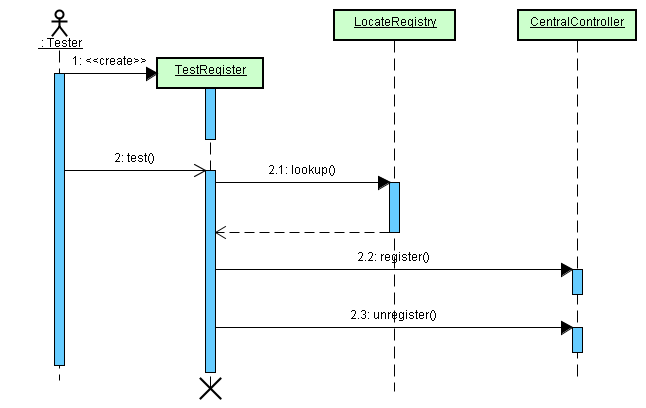
\includegraphics[width=\textwidth]{img/tests/testRegister2.png}
	\caption{Test Case: TestRegister}
	\label{fig:resolution_2}
\end{figure}
Opis:
\begin{enumerate}
	\item create()\\
	Stworzenie obiektu klasy TestRegister
	\item test()\\
	Tester wywoluje na stworzonym obiekcie metod� test()
	
		\begin{enumerate}
			\item lookup()\\
			TestRegister wyszukuje w LocateRegistry obiektu CentralController
			\item register()\\
			Klasa TestRegister rejestruje si� w CentralController
			\item unregister()\\
			Klasa TestRegister wyrejestrowuje si� z CentralController
		\end{enumerate}
\end{enumerate}
\subsubsection{Wyniki}
\begin{center}
\begin{tabular}{|l|l|l|}
\hline  
\textbf{Clients} & \textbf{Mean Time}& \textbf{Errors} \\
\hline 
10 & 2777 & 0\\
\hline
20 & 2829 & 0\\
\hline
30 & 4914 & 0\\
\hline
40 & 6014 & 0\\
\hline
50 & 6279 & 0\\
\hline
60 & 6937 & 0\\
\hline
70 & 7819 & 0\\
\hline
80 & 8948 & 0\\
\hline
90 & 9458 & 0\\
\hline
100 & 10953 & 0\\
\hline
110 & 11545 & 0\\
\hline
120 & 12496 & 0\\
\hline
130 & 15927 & 0\\
\hline
140 & 16322 & 0\\
\hline
150 & 16729 & 0\\
\hline
160 & 29865 & 7\\
\hline
170 & 27012 & 8\\
\hline
180 & 30328 & 14\\
\hline
190 & 33825 & 19\\
\hline
200 & 34480 & 27\\
\hline
\end{tabular}  
\end{center}
Nie by�o sensu liczy� dalej, gdy� b��dy mia�y znaczny wp�yw na wyniki i psu�yby wykresy zale�no�ci czasu oczekiwania od liczby uruchomionych w�tk�w klienckich. Te b��dy objawia�y si� w logach jako ConnectionRefused. S�dzimy, �e jest to zwi�zane z pul� w�tk�w RMI. 
\begin{figure}[h]
	\centering
		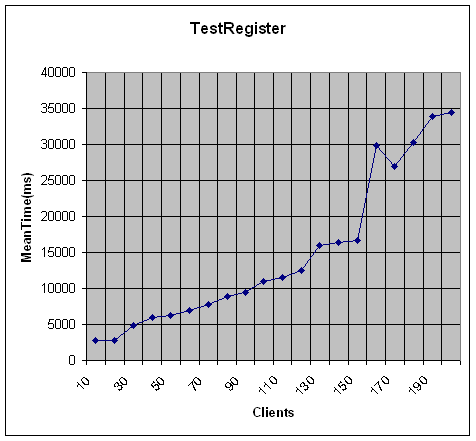
\includegraphics[width=\textwidth]{img/tests/testRegister-results2.png}
	\caption{TestRegister: Results}
	\label{fig:resolution_2}
\end{figure}

%\section{Bezpiecze�stwo}

\subsection{Miejsca nara�one na ataki}
\subsubsection{Sie�}
Obliczenia sieciowe s� zorganizowane na bazie architektury klient-serwer zrealizowanej za pomoc� RMI, klienci rejestruj� swoj� gotowo�� do prowadzenia oblicze� na serwerze, nast�pnie serwer posy�a ka�demu z klient�w zadanie do wykonania. Nast�pnie klient sprawdza w bazie danych jakie pluginy s� mu potrzebne do wykonania zadania oraz �ci�ga je ze znalezionego adresu URL. Serwer, co pewien czas, pyta o klient�w o wyniki.\\

\begin{figure}[h]
	\centering
		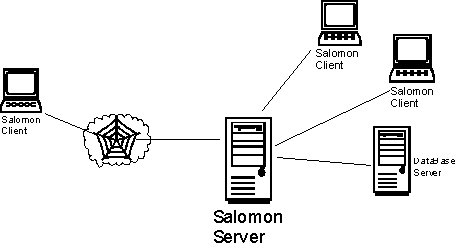
\includegraphics[width=\textwidth]{img/security/nofirewall.png}
	\caption{Architektura}
	\label{fig:arch}
\end{figure}

Pierwszym problemem bezpiecze�stwa jest brak kontroli nad tym kto mo�e si� po��czy� jako klient. Poniewa� po po��czeniu, wszystkie metody s� wywo�ywane przez serwer na kliencie nie wzrasta w ten spos�b podatno�ci na ataki DOS a podatno�� na Synflood jest taka jak ca�ego systemu , mimo to stanowi to zagro�enie dla sp�jno�ci oblicze� poniewa� fa�szywy klient mo�e zwraca� niepoprawne wyniki zar�wno ze wzgl�du na warto�ci nie oczekiwane przez program, co mo�e spowodowa� zawieszenie w przypadku  b��du w serwerze, jaki i dane niepoprawne merytorycznie co zak��ci przebieg obliczenia. Sugerowan� metod� przeciwdzia�ania by�o by wprowadzenie list dost�pu na serwerze lub ich implementacja na firewallu. Mo�na ewentualnie wprowadzi� has�a przy logowania ale ich u�yteczno�� by�a by znikoma poniewa� klient a nie serwer udost�pnia tutaj zasoby (chyba �e komu� mog�o by zale�e� na kradzie�y tej porcji danych kt�ra zostanie wys�ana klientowi).\\

\begin{figure}[h]
	\centering
		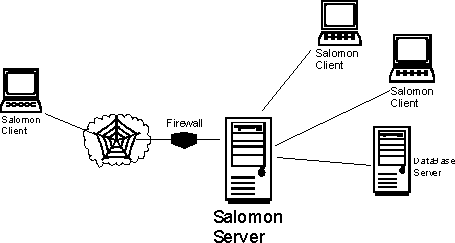
\includegraphics[width=\textwidth]{img/security/firewall.png}
	\caption{Rozwi�zanie 1}
	\label{fig:resolution_1}
\end{figure}
          
Istnieje mo�liwo�� przeprowadzenia ataku DOS je�li metoda klienta odpowiedzialna za przyj�cie zadania do wykonania wejdzie w niesko�czon� p�tl�. W�tek serwera b�dzie czeka� na powr�t metody od klienta co w przypadku zmasowanych po��cze� tak spreparowanych klient�w mo�e doprowadzi� do wyczerpania puli w�tk�w co spowoduje �e serwer nie b�dzie przyjmowa� nowych po��cze�. Nie mo�emy si� ca�kowicie obroni� przed tego typu atakiem ale mo�emy znacznie ograniczy� szkody nim wywo�ane poprzez wprowadzanie timeout�w dla w�tk�w obs�ugi klient�w b�d�cych w stanie oczekiwania na odpowied� od klienta.\\

Nast�pnym mo�liwym problemem jest pobieranie listy plugin�w z bazy danych. Atakuj�cy potrafi�cy z�ama� zabezpieczenia bazy danych b�d� porwa� po��czenie, jest wstanie wskaza� swoje w�asne �r�d�o plugin�w co mo�e doprowadzi� do wykonania obcego kodu u klienta. Na zapewnienie bezpiecze�stwa bazie danych mamy wp�yw tylko �rodkami og�lnosystemowymi. Zalecane jest jednak aby tunelowa� po��czenie do bazy poprzez szyfrowane po��czenie co utrudni jego przechwycenie raz zdobycie has�a do bazy. Mo�liwo�ci wykonania obcego kodu s� ograniczone przez maszyn� wirtualn� javy i b�d� om�wione w rozdziale dotycz�cym bezpiecze�stwa lokalnego.

\begin{figure}[h]
	\centering
		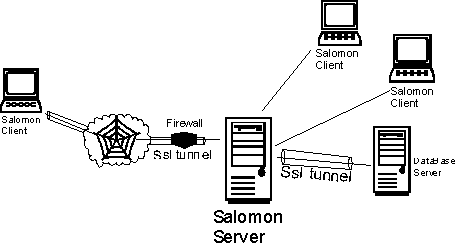
\includegraphics[width=\textwidth]{img/security/ssl.png}
	\caption{Rozwi�zanie 2}
	\label{fig:resolution_2}
\end{figure}

\subsubsection{U�ytkownik lokalny}
Wi�kszo�� spraw bezpiecze�stwa wykonania kodu jest kontrolowana przez �rodowisko tj. Wirtualn� Maszyn� Javy. Odpada dzi�ki temu ca�kiem spora klasa atak�w typu buffer overflow, Zakresy tablic s� kontrolowane przez Jav� co nie pozwala na wyj�cie poza swoj� pami�� i nadpisanie stosu. Dzi�ki odpowiednio ustawionej polityce bezpiecze�stwa maszyny wirtualnej mo�emy zabroni� jakichkolwiek pr�b komunikacji plugin�w ze �rodowiskiem. 
Bardzo wa�nym jest aby zabroni� pluginom wi�kszo�ci rzeczy z grupy runtime tak jak �adowanie bibliotek z natywnym kodem (praktycznie nieograniczone mo�liwo�ci), zamkni�cia maszyny (denial-of-service), tworzenia w�asnych ClassLoader�w (Wykonanie niebezpiecznego kodu) czy ustawiania w�asnych fabryk dla gniazd (Mo�liwo�� podmiany implementacji gniazda a co za tym idzie zmiana danych kt�re przez nie przechodz�). Ca�ej aplikacji musi by� wolno u�ywa� JDBC oraz otwiera� gniazda, pluginy b�d� korzysta�y tylko z klas engine'u salomona wiec i tej funkcjonalno�ci nie potrzebuj�.
\newpage

\subsection{Propozycje bezpiecznej konfiguracji}
Jak wida� zagro�e� jest wiele, jednak ca�e �rodowisko obliczeniowe by�o projektowane z my�l� o uruchomieniu go w sieci odseparowanej od internetu b�d� poprzez VPN a przy takim opakowaniu wymienione luki staj� si� ma�o gro�ne, nie mo�emy jednak polega� na bezpiecze�stwie opartym na niewiedzy o lukach gdy� w przypadku w�amania do wewn�trz sieci mog� stanowi� one cel atak�w.
\subsubsection{Plik salomon.policy}
Plik salomon.policy okre�la prawa kodu do wykonania potencjalnie niebezpiecznych dla u�ytkownika akcji 
oraz wszelkich dzia�a� poza "`piaskownic�"' maszyny wirtualnej Javy. Projekt posiada wie domeny bezpiecze�stwa, jedn� dla kodu samego salomona, drug� o wiele bardziej restrykcyjn� dla plugin�w u�ytkownik�w. 

\begin{verbatim}
grant codeBase "file:/${installdir}/bin" {
  permission java.awt.AWTPermission "listenToAllAWTEvents";
  permission java.io.FilePermission "${installdir}${/}-", "read, write";
  permission java.lang.RuntimePermission "createClassLoader";
  permission java.lang.RuntimePermission "exitVM";
  permission java.sql.SQLPermission "setLog";
  permission java.util.PropertyPermission "*", "read";
  permission java.awt.AWTPermission "showWindowWithoutWarningBanner";
  permission java.lang.RuntimePermission "loadLibrary.*";
  permission java.lang.RuntimePermission "shutdownHooks";
  permission java.lang.RuntimePermission "stopThread";
  permission java.util.logging.LoggingPermission "control";
};


\end{verbatim}

Poniewa� engine zajmuje si� po��czeniami z baz� danych oraz obs�ug� sieci, domenie \texttt{bin/} zosta�y przydzielone pozwolenia na korzystanie z sieci, dodatkowe dla JDBC,  zezwolenie na �adowanie bibliotek natywnych oraz ustawianie logowanie SQLa. Bardzo wa�nym jest przydzielenie pozwole� z klasy Runtime. Engine zajmuje si� �adowanie plugin�w z sieci wi�c potrzebny mu jest w�asny ClassLoader, zosta�o wiec  przydzielone pozwolenie "`createClassLoader"', dodatkowo przydzielono zezwolenia na zamkni�cie maszyny oraz na kontrole nad w�tkami, pozwolenie to jest szczeg�lnie przydatne podczas kontroli klient�w oczekuj�cych na w�tkach. Zezwolenia na u�ycie AWT pozwol� na wy�wietlenie GUI
\begin{verbatim}
grant codeBase "file:/${installdir}/plugins" {
  permission java.awt.AWTPermission "listenToAllAWTEvents";
  permission java.awt.AWTPermission "showWindowWithoutWarningBanner";
};


\end{verbatim}
Pluginom ze wzgl�d�w bezpiecze�stwa zosta�o zabrane wi�kszo�� pozwole�. Pluginy same wy�wietlaj� swoje GUI z  konfiguracj� wi�c potrzebuj� zezwolenie na u�ycie AWT. Jednak�e danie im zezwole� na wszelkie akcje z klasy Runtime by�o by wysoce niebezpieczne poniewa� szkodliwy plugin m�g� by za�adowa� swoje klasy z poza domeny i tym samy obej�� wszystkie zabezpieczenia




\newpage
\section{Dalszy rozw�j systemu}
\begin{itemize}
\item Stworzenie automatycznych nocnych test�w. Powinien zosta� stworzony skrypt, kt�ry sprawdza czy danego dnia by�y jakie� zmiany pod kontrol� wersji i w razie zmian przeprowadza proces budowania instalki i odpalania test�w. Testowanie jednostkowe przeprowadzane b�dzie na �r�d�ach, natomiast testowanie GUI na wersji zainstalowanej, ale z binari�w skompilowanych z kontraktami (sprawdza�oby to instalator oraz kontrakty)
\item Dodanie batchmode - stworzenie nowego kontrolera, kt�ry konfiguracj� oraz zadania wczytywa�by z plik�w xml.  Pozwoli�oby to na tworzenie zada� dla Salomona przez inne programy poprzez generowanie odpowiedniego xml'a. Batchmode m�g�by by� r�wnie� wykorzystywany do test�w regresyjnych - sprawdzane by by�o czy dla danego pliku xml wynik jest zawsze ten sam 
\item Podzielenie plugin�w na kategorie w hierarchii drzewiastej - drzewiasta hierarchia jest bardziej naturalna. (np. pluginy to wyszukiwania klastr�w, pluginy do wyszukiwania regu�).
\item Automatyczne rozmieszczanie zada� pomi�dzy r�nych klient�w. Tworzone zadana powinny by� przedstawiane w spos�b graficzny jako graf (acykliczny), gdzie ka�dy w�ze� odpowiada�by pojedynczemu zadaniu. Podzia� zada� na hosty powinien by� automatyczny i dynamiczny (tzn. optymalizowa� si� w trakcie wykonania). Obecny interfejs \emph{ServerController} powinien by� wykorzystywany do �ledzenia wykonywania zada�, na grafie ka�dy w�ze� powinien zawiera� informacje, na kt�rym aktualnie kontrolerze zadanie si� wykonuje oraz jego status.
\item Dodanie nowych menad�er�w (obs�uga r�nych typ�w wiedzy)
\item Mechanizm dodawania/modyfikacji menad�er�w jako wtyczek (mechanizm ten nie musi by� dynamiczny z racji ze nowe menad�ery tworzone b�d� niezwykle rzadko)
\item Dodanie nowych wtyczek
\item Konfiguracja programu z poziomu interfejsu u�ytkownika
\item Statystyki: Ilo�� zada�, ilo�� zada� o danym statusie wykonania, statystyki dotycz�ce ka�dego typu danych przechowywanego w bazie (klastry, atrybuty, itp.). Statystyki powinny by� tworzone per ka�de odpalenie listy zada� oraz w ca�ej historii, statystyki powinny by� prezentowane w formie graficznej. Dzi�ki statystykom u�ytkownik mia�by mo�liwo�� obserwowania zmian w zgromadzonej wiedzy.
\item Bardzo wa�nym zdaniem jest wprowadzenie mo�liwo�ci importu oraz synchronizacji danych z innych baz. Baza na kt�rej operuje ka�da instancja Salomona jest jego wewn�trzn� baza, zatem dane te w kontek�cie ca�ego systemu powinny by� synchronizowane. Brak tej funkcjonalno�ci uniemo�liwia zastosowanie systemu w �rodowiskach produkcyjnych
\item Stworzenie uniwersalnych komponent�w do prezentacji wspieranych typ�w danych. Komponenty te wykorzystywane by�yby zar�wno do prezentowania aktualnie zgromadzonej wiedzy jak r�wnie� mog�yby by� wykorzystywane przez wtyczki. Dzi�ki takiemu podej�ciu warstwa prezentacji danych by�aby bardziej sp�jna.
\end{itemize}

\section{Odno�niki}
\begin{itemize}
\item \emph{Java} (\href{http://java.sun.com}{http://java.sun.com})
\item \emph{Firebird} (\href{http://firebird.sourceforge.net}{http://firebird.sourceforge.net})
\item \emph{Subversion} (\href{http://subversion.tigris.org}{http://subversion.tigris.org})
\item \emph{Eclipse} (\href{http://www.eclipse.org}{http://www.eclipse.org})
\item \emph{Ant} (\href{http://ant.apache.org}{http://ant.apache.org})
\item \emph{Log4j} (\href{http://logging.apache.org/log4j}{http://logging.apache.org/log4j})
\item \emph{IzPack} (\href{http://www.izforge.com/izpack}{http://www.izforge.com/izpack})
\item \emph{JUnit} (\href{http://www.junit.org}{http://www.junit.org})
\item \emph{Abbot} (\href{http://abbot.sourceforge.net}{http://abbot.sourceforge.net})
\end{itemize}


\end{document}
